\documentclass[a4paper,12pt]{article}
\usepackage[utf8]{inputenc}
\usepackage[T1]{fontenc}
\usepackage[italian]{babel}
\usepackage{geometry}
\usepackage{lmodern}
\usepackage{amsmath,amssymb}
\usepackage{enumitem}
\usepackage{hyperref}
\usepackage{listings}
\usepackage{xcolor}
\usepackage{graphicx}
\usepackage{pgfplots}
\usepackage{fancyhdr}
\usepackage{titlesec}
\usepackage{graphicx}
\titleformat{\section}
  {\normalfont\Large\bfseries\centering}  % Format: font size, bold, centered
  {\thesection}{1em}{} 
\pagestyle{fancy}
\pgfplotsset{compat=1.18}
\fancyhead{}
\fancyfoot{}
\fancyhead[L]{Gabriele Perna}          % Left side
\fancyhead[C]{Programmazione e algoritmica}     % Center
\fancyhead[R]{2025/2026}             % Right side
\fancyfoot[C]{\thepage}           % Page number in the center of footer
\let\oldsection\section
\renewcommand{\section}{\clearpage\oldsection}
\geometry{margin=2.5cm}

\title{Programmazione e Algoritmica}
\author{}
\date{}

\begin{document}

\maketitle
\tableofcontents
\section{Concetti Iniziali}

Uno dei primi scopi dell’algoritmica è utilizzare al meglio le informazioni che si hanno.
\begin{itemize}
  \item \textbf{Algoritmo}: sequenza di istruzioni non ambigua che, dati in input, produce un output corretto.
  \item \textbf{Programma}: implementazione di un algoritmo in un linguaggio preciso, non ambiguo e formalmente definito. Eseguibile da una macchina
  \item \textbf{Tipo}: insieme dei valori assumibili da una variabile.
\end{itemize}
Per ogni problema esistono infiniti algoritmi per risolverlo e quindi infiniti programmi.\\\\
La maggior parte degli algoritmi assume una forma astratta per adattarsi a varie situazioni che possono essere risolte con metodologie simili.

\paragraph{Obiettivi della programmazione:}
\begin{itemize}
  \item Efficienza
  \item Correttezza
  \item Velocità di coding (efficienza nel tempo impiegato dai developer)
  \item Manutenibilità
\end{itemize}

\section{Strutture Dati}

\begin{itemize}
  \item \textbf{Variabile}: singola cella di memoria che contiene un valore.
  
  \item \textbf{Array}: sequenza di celle contigue, accessibili direttamente tramite indice.
  
  \item \textbf{Lista collegata}: insieme di nodi in cui ogni elemento contiene un valore e un riferimento al successivo.
  
  \item \textbf{Pila (stack)}: struttura LIFO (Last In, First Out); l’ultimo elemento inserito è il primo ad essere rimosso.
  
  \item \textbf{Coda (queue)}: struttura FIFO (First In, First Out); il primo elemento inserito è il primo ad essere rimosso.
  
  \item \textbf{Albero}: struttura gerarchica composta da nodi collegati da archi, con un nodo radice.
  
  \item \textbf{Heap}: particolare tipo di albero binario (quasi completo) che soddisfa la proprietà di heap (min-heap o max-heap).
  
  \item \textbf{Grafo}: insieme di nodi (vertici) collegati da archi; può essere orientato o non orientato.
  
  \item \textbf{Tabella hash}: struttura che associa chiavi a valori tramite una funzione hash, permettendo accessi molto rapidi in media.
\end{itemize}

\section{Linguaggi formali}

Un linguaggio detto \textbf{formale} ha:
\begin{itemize}
  \item \textbf{Sintassi}: struttura grammaticale (correttezza grammaticale).
  \item \textbf{Semantica}: significato (correttezza logica).
\end{itemize}

Ogni linguaggio di programmazione è un linguaggio formale.

\section{Storia degli Algoritmi}

Il concetto di algoritmo ha origini molto antiche: già nelle prime civiltà si utilizzavano procedure sistematiche per risolvere problemi matematici e pratici.

Nell’antico Egitto e in Mesopotamia esistevano metodi per eseguire operazioni aritmetiche e risolvere equazioni. Un esempio importante è l’algoritmo di Euclide (III secolo a.C.), utilizzato per calcolare il massimo comune divisore tra due numeri, uno dei più antichi algoritmi ancora in uso.

Nel Medioevo, un contributo fondamentale fu dato da \textbf{Leonardo Fibonacci}, che nel suo libro \textit{Liber Abaci} (1202) diffuse in Europa il sistema numerico indo-arabico. Questo sistema posizionale rese possibili algoritmi di calcolo molto più efficienti rispetto ai numeri romani.

Il termine “algoritmo” deriva dal nome del matematico persiano \textbf{Al-Khwarizmi} (IX secolo), i cui lavori introdussero metodi sistematici per il calcolo e la risoluzione di problemi matematici.

Nel XIX secolo, \textbf{Charles Babbage} progettò la “macchina analitica”, considerata un precursore del computer moderno, mentre \textbf{Ada Lovelace} scrisse quello che è spesso considerato il primo programma della storia.

Nel XX secolo si ebbe la formalizzazione teorica del concetto di algoritmo grazie a studiosi come \textbf{Alan Turing}, che introdusse la macchina di Turing, un modello astratto di calcolo fondamentale per l’informatica teorica. Nello stesso periodo nacquero i primi computer elettronici e i primi linguaggi di programmazione.

Con lo sviluppo dell’informatica, gli algoritmi sono diventati sempre più centrali, trovando applicazione in ambiti come la crittografia, l’intelligenza artificiale, l’analisi dei dati e la ricerca operativa.

Infine, è interessante osservare che anche in natura esistono sistemi che codificano e trasmettono informazioni, come il DNA, che può essere visto come un sistema di istruzioni biologiche.
\section{Alfabeti}

\subsection{Definizione di alfabeto}

Un \textbf{alfabeto} è un insieme finito di simboli.\\
Una \textbf{stringa} è una sequenza di simboli di uno specifico alfabeto (anche con ripetizioni) e ha lunghezza finita.  
Può anche essere vuota, con lunghezza 0, indicata con $\varepsilon$.

\[
|baco| = 4 \quad \text{se} \quad a = \text{"baco"}
\]
Un linguaggio $L$ su un alfabeto $A$ è sottoinsieme di $A^*$ (tutte le possibili combinazioni dell’alfabeto).\\
Descrivere un linguaggio di programmazione significa descrivere quali frasi sono ammissibili.\\
Si usano le regole di una grammatica e un metodo riconoscitivo per la semantica.

\subsection{Grammatica di un alfabeto}

La grammatica è una tripla $(T, N, P)$ dove:
\begin{itemize}
  \item $T$ = simboli terminali (alfabeto di riferimento)
  \item $N$ = simboli non terminali
  \item $P \subseteq S \times S^*$ = insieme delle produzioni, con $S = T \cup N$
\end{itemize}

\subsection{Derivativo immediato}

Data una grammatica $G(T, N, P)$, si dice che $\beta_1$ è \textbf{derivativo immediato} di $\beta$ se è possibile ottenere $\beta_1$ da $\beta$ applicando una produzione.

\[
\beta = \beta_1 X \beta_2, \quad X \in N
\]
Esempio:
\[
\beta = Exp + Exp\, Op\, 2
\]
Produzione: $Exp ::= Num$
\[
\Rightarrow \beta_1 = Num + Exp\, Op\, 2
\]

\subsection{Derivativo}

È come il derivativo immediato, ma ottenuto tramite $N$ sostituzioni.

\subsection{Linguaggio generato}

Data $G(T,N,P)$ e $X \in N$, il linguaggio di $X$, scritto $L(X)$, è l’insieme di tutti e soli i derivativi $\beta \in T^*$ di $X$.

\[
L(X) = \{w \mid w \in T^*, X \Rightarrow^* w\}
\]
Esempio:
\[
B ::= 1 \;|\; 0B \;|\; 1B
\]
Stringhe che finiscono con 1.

\[
B \Rightarrow 1B \Rightarrow 10B \Rightarrow 100B \Rightarrow 1001
\]
“1001” appartiene al linguaggio, “1000” no.

\subsection{Derivazioni canoniche}

\begin{itemize}
  \item \textbf{Sinistra}: si sostituisce sempre il simbolo più a sinistra.
  \item \textbf{Destra}: si sostituisce sempre quello più a destra.
\end{itemize}

\subsection{Alberi di derivazione (Parse Trees)}

Rappresentano tutti i possibili percorsi per effettuare una derivazione (insiemi $N$ e $E$: nodi e archi).  
Non possono esserci due o più archi verso lo stesso nodo e il nodo radice non ha archi entranti.

\section{Regole di Inferenza}

Per definire la semantica del linguaggio MAO si usano \textbf{regole di inferenza}.

\[
\frac{P_1, \dots, P_n}{Q}
\]
Se tutte le premesse $P_i$ sono vere, $Q$ è vero.\\  
Se non ci sono premesse, abbiamo un \textbf{assioma} (sempre vero).\\\\
Un sistema logico è un insieme di regole di inferenza per dimostrare la validità di formule.\\
La derivazione nel sistema logico è una sequenza di passaggi che parte dagli assiomi e giustifica una conclusione.
\[
D \vdash G
\]
\textbf{Condizioni laterali}: condizioni aggiuntive che devono essere soddisfatte oltre alle premesse.\\
In un linguaggio logico, ogni produzione grammaticale ha una regola di inferenza collegata.

\section{Efficienza e costo computazionale}

Si misura in base a:
\begin{itemize}
  \item Costo in tempo d’esecuzione (numero di operazioni elementari, ovvero non affette dal variare dell'input)
  \item Costo in memoria (celle utilizzate)
\end{itemize}
Il costo (tempo/spazio) si esprime in \textbf{ordine di grandezza}, considerando solo il termine dominante.\\
La somma di due costi costanti, ovvero legati ad operazioni elementari, è un costo costante.\\\\
Il costo totale di un algoritmo / programma può essere rappresentato sotto forma di funzione su piano cartesiano in cui l'incognita corrisponde all'input.\\\\
La complessità è una \textbf{funzione di n}, con n come input variabile.\\
Per vedere se una funzione / algoritmo è più \textbf{veloce} si applicano le operazioni degli infinitesimi tipiche dell'analisi matematica.
\subsection{O, $\Omega$, $\Theta$}
\paragraph{O grande: } si usa per indicare il limite asintotico superiore della funzione della complessità (non può mai essere maggiore).\\
La definizione di O grande significa che per un valore abbastanza grande di $n$ (input) esiste un $c$ per cui la funzione della complessità si troverà sempre al di sotto di O grande.
\paragraph{$\Omega$ grande: } si usa per indicare il limite asintotico inferiore della funzione della complessità (non può scendere al di sotto).
La definizione di $\Omega$ grande significa che per un valore abbastanza grande di $n$ esiste un $c$ per cui la funzione della complessità si troverà sempre al di sopra di $\Omega$ grande. 
\paragraph{$\Theta$ grande: } quando limite superiore e inferiore coincidono, si ha $\Theta$ grande. Ciò vuol dire che la funzione della complessità si trova schiacciata tra il limite superiore e inferiore (\textbf{Teorema dei carabinieri}). Attenzione, ciò non vuol dire che le $c$ delle due condizioni siano uguali.\\\\
Con "$c$" intendiamo una costante moltiplicata al limite inferiore o superiore.

$\Gamma_1[\Gamma_2]$

\paragraph{Esempio: } dimostrare:
\[
3n^2 - 2n - 1 \in \Theta(n^2)
\]
Bisogna trovare il valore delle $c$ che soddisfano entrambi le condizioni:
\[
C_1 (n^2) \le 3n^2 - 2n - 1 \le C_2 (n^2)
\]
\textbf{C1 = } 2.\\
\textbf{C2 = } 3, dato che la funzione è simile, escluso il fatto che viene anche sottratto qualcosa (- 2n - 1).

\subsection{Teorema Principale (Master Theorem)}

Si consideri una ricorrenza della forma
\[
T(n) = a\,T\!\left(\frac{n}{b}\right) + f(n),
\]
dove $a \ge 1$ (numero chiamate ricorsive), $b > 1$ (indice di riduzione del problema) e $f(n)$ è una funzione asintoticamente positiva (complessità di ogni chiamata).
Sia
\[
n^{\log_b a}
\]
il costo indotto dalla parte ricorsiva dell'algoritmo.\\
Il Teorema Principale permette di determinare l'ordine di crescita di $T(n)$
confrontando $f(n)$ con $n^{\log_b a}$. Sono possibili tre casi.

\subsection{Caso 1: $\;f(n)$ cresce meno della ricorsione}
Se esiste $\epsilon > 0$ tale che
\[
f(n) = O\!\left(n^{\log_b a - \epsilon}\right),
\]
allora
\[
T(n) = \Theta\!\left(n^{\log_b a}\right).
\]

\subsection{Caso 2: $\;f(n)$ cresce come la ricorsione}
Se esiste $k \ge 0$ tale che
\[
f(n) = \Theta\!\left(n^{\log_b a}\,\log^{k} n\right),
\]
allora
\[
T(n) = \Theta\!\left(n^{\log_b a}\,\log^{k+1} n\right).
\]

\subsection{Caso 3: $\;f(n)$ cresce più della ricorsione}
Se esiste $\epsilon > 0$ tale che
\[
f(n) = \Omega\!\left(n^{\log_b a + \epsilon}\right),
\]
e se vale la condizione di regolarità
\[
a\, f\!\left(\frac{n}{b}\right) \le c\, f(n)
\qquad \text{per qualche } c < 1,
\]
allora
\[
T(n) = \Theta\!\left(f(n)\right).
\]

\bigskip

\noindent
In sintesi, il Teorema Principale permette di risolvere molte ricorrenze
della forma $T(n) = a T(n/b) + f(n)$ confrontando il costo ricorsivo
$n^{\log_b a}$ con il costo non ricorsivo $f(n)$.

\subsection{Metodo iterativo}
Quando non si riesce ad applicare il teorema principale si può usare il \textbf{metodo iterativo}.\\
Col metodo iterativo bisogna proseguire come per induzione:
\begin{center}
  \begin{align*}
    T(n) &= T(n-1) + C_1\\
    T(n) &= T(n-2) + C_1 + C_2\\
    T(n) &= T(n-3) + C_1 + C_2 + C_3\\
    ...
  \end{align*}
\end{center}
Si termina con il caso base, ovvero $n-1 = 1 = C_0$


\subsection{Alberi di ricorsione}
Quando non si riesce ad applicare il teorema principale si possono usare gli \textbf{alberi di ricorsione}.\\
Si svolge comunque la ricorsione ma si disegna una specie di albero discendente laterale, indicando ogni volta $f(n)$ per ogni step.\\
Il valore finale, se l'esempio è uguale a quello del metodo iterativo, sarà $f(n) \cdot $ numero di chiamate iterative.

\paragraph{Fooling argument: }un algoritmo deve leggere tutti gli input per svolgere u bel lavoro, infatti se abbiamo $n$ input si ha una complessita minima di $n$ ($\Omega n$)\\
Questo vale solo quando non ci sono ipotesi particolari sui dati in input, come ordinamento.

\section{Programmazione dinamica}
La \textbf{programmazione dinamica} (PD) è una tecnica di progettazione di algoritmi. Come il divide-et-impera, è una tecnica che si applica nei casi in cui
la soluzione del problema può essere definita ricorsivamente.\\
A differenza del divide-et-impera però, che opera in maniera top-down fino a ridursi a sottoproblemi via via più piccoli, la PD risolve prima i sottoproblemi e poi in maniera \textbf{bottom-up} a partire dalla loro soluzione costruisce via via soluzioni a sottoproblemi più grandi fino al problema originale.\\\\
Ecco gli step da eseguire per sviluppare un algoritmo con la programmazione dinamica:
\begin{itemize}
    \item Identificare i sottoproblemi "interessanti".
    \item Identificare e risolvere in modo \textbf{diretto} i sottoproblemi elementari.
    \item Stabilire la regola ricorsiva per il calcolo della soluzione dei sottoproblemi e dei problemi soprastanti a partire dai valori gia calcolati.
    \item Capire come restituire il valore del problema generale.
\end{itemize}
Vediamo un esempio con il calcolo dell'n-esimo numero di fibonacci.
\[
f(0) = 0
\]
\[
f(1) = 1
\]
\[
f(n) = f(n-1) + f(n-2)
\]
\begin{lstlisting}
    fibRec(n) { //Versione ricorsiva
        if (n = 0): return 0
        if (n = 1): return 1
        return fibRec(n-1) + fibRec(n-2)
    }
\end{lstlisting}
Lo stesso problema in PD svolge i casi base e \textbf{ricorsivamente} risolve i casi superiori fino ad arrivare ad n.
\begin{lstlisting}
    fibPD(n) {
        f = []
        f[0] = 0
        f[1] = 1
        for (i = 2, i <= n, i++):
            f[i] = f[i-1] + f[i-2]
        return f[n]
    }
\end{lstlisting}
Vediamo adesso un'altro problema: abbiamo una corda lunga $n$ cm e una tabella di prezzi, ogni prezzo è relativo a una lunghezza specifica. Calcolare il ricavo massimo ottenibile tagliando la corda.\\
Nel caso avessimo una corda di $4$ cm, e questi prezzi:
\[
\begin{bmatrix}
    1cm = 1\\
    2cm = 5\\
    3cm = 8\\
    4cm = 9\\
\end{bmatrix}
\]
La corda può essere tagliata in $2^{n-1}$ modi.\\
La \textbf{soluzione ottima} è due sotto-corde da $10cm$, vediamo come trovarlo tramite un programma:\\
Soluzione ricorsiva:
\begin{lstlisting}
    ropeCut(p,n)  {\\prezzi e lunghezza corda
        if(n=0): return 0
        q = -infty
        for (i=1,i<=n,i++):
            q = max(q,p[i] + ropeCut(p,n-1))
        return q
    }
\end{lstlisting}
Soluzione PD:
\begin{lstlisting}
    ropeCut(p,n):
        r = []
        r[0] = 0
        for (j = 1 to n):
            q = -inf
            for (i = 1 to j):
                if (q < p[i] + r[j-1]):
                    q = p[i] + r[j-1]
            r[j] = q
        return r[n]
\end{lstlisting}
\subsection{Esercizi}
\subsubsection{Problema 1 (Dello zaino)}
Si mostri la tabella per la risoluzione del problema zaino 0-1 per l'istanza:
\[
\begin{bmatrix}
    Oggetto & Peso & Valore\\
    a & 1 & 60\\
    b & 2 & 100\\
    c & 3 & 120
\end{bmatrix}
\]
Lo spazio a disposizione è 5.\\
Usiamo una matrice T$(n+1) X (w+1)$, ogni cella $T_{ij}$ corrisponde al peso totale trasportabile avendo $j$ come massimo peso totale e i primi $i$ oggetti.
\[
T[i,0] = T[0,j] = 0
\]
\[
T[i,j] = \begin{cases}
    T[i-1,j] \impliedby P[i] > j\\
    max(T[i-1,j],v[i] + T[i-1,j - p[i]]) \impliedby P[i] \leq j
\end{cases}
\]
Per esempio vediamo il caso per $w = 1$ e $n = 1$ (n indica quanti oggetti, a partire dal primo, sono disponibili):
\[
T[1,1] = 60
\]
Prende il secondo caso, perche rientra nel peso possibile.\\
Vediamo la tabella completa:
\[
\begin{bmatrix}
    N / W & 0 & 1 & 2 & 3 & 4 & 5\\
    0 & 0 & 0 & 0 & 0 & 0 & 0\\
    1 & 0 & 60 & 60 & 60 & 60 & 60 \\
    2 & 0 & 60 & 100 & 160 & 160 & 160\\
    3 & 0 & 60 & 100 & 160 & 180 & 220
\end{bmatrix}
\]
L'output finale è $220$, con un peso massimo di $5$ e tale catalogo di oggetti posso portare dietro un massimo valore di $220$.
\subsubsection{Problema 2 (Del viaggiatore)}
Un viaggiatore ha una valigia di capacità C e un insieme di $n$ souvenir, il cui volume è $v[i]$. Qual'è il minimo numero di souvenir che riempiono la valigia esattamente?\\
Osserviamo che il problema è simile al precedente, ma il valore non è da massimizzare, bensì da minimizzare.
\[
V = \begin{bmatrix}
    2 & 2 & 4 & 3 & 1
\end{bmatrix}
\]
\[
N = 5
\]
\[
W = 7
\]
L'output è ovviamente $V[3] + V[4] = 4 + 3$ e quindi $2$ oggetti, ma vediamo come progettare un algoritmo che risolve tale problema.\\
Si opera proprio come nel problema dello zaino:
\[
\Pi_{n,w} = \text{problema iniziale}
\]
\[
\Pi_{i,j} = \text{sottoproblema con i oggetti e capacità j, }0 \leq i \leq n, 0 \leq j \leq w
\]
Per sottostruttura ottima, il problema generale contiene la soluzione del sottoproblema.\\
Vediamo la tabella di output generata:
\[
T[0,j] = +\infty
\]
Dato che non si hanno oggetti e quindi di default si mette tale valore, è impossibile riempire la valigia.
\[
T[i,0] = 0
\]
Dato che non si può riempire una valigia che non può contenere neanche un oggetto di peso minimo, è come se fosse "gia riempita"
\[
T[i,j] = \begin{cases}
    M[i-1,j] \impliedby j < v[i]\\
    min(T[i-1,j],1 + T[i-1,j-v[i]])
\end{cases}
\]
\[
\begin{bmatrix}
    N / W & 0 & 1 & 2 & 3 & 4 & 5 & 6 & 7\\
    0 & 0 & +\infty & +\infty & +\infty & +\infty & +\infty & +\infty & +\infty\\
    1 & 0 & +\infty & 1 & +\infty & +\infty & +\infty & +\infty & +\infty\\ 
    2 & 0 & +\infty & 1 & +\infty & 2 & +\infty & +\infty & +\infty\\  
    3 & 0 & +\infty & 1 & +\infty & 1 & +\infty & 2 & +\infty\\ 
    4 & 0 & +\infty & 1 & 1 & 1 & 2 & 2 & 2\\
    5 & 0 & 1 & 1 & 1 & 1 & 2 & 2 & 2\\
\end{bmatrix}
\]
\subsubsection{Problema 3 (Come passare l'esame)}
Si consideri un esame con $n$ problemi, ognuno dei quali vale $P[i]$ punti e si richiede $t[i]$ minuti per essere svelto. L'obiettivo è passare l'esame con il minimo sforzo possibile (tempo).\\
Si vuole quindi passare l'esame con il minor tempo possibile, il voto deve essere almeno sopra una soglia V quindi.\\
Progettare e descrivere in pseudocodice un algoritmo PD che, dati i vettori P e t e la soglia V, trovi il sottoinsieme di problemi che richiede il minimo tempo totale che faccia passare l'esame.\\
Inoltre, simulare l'algoritmo sui dati:
\[
P = \begin{bmatrix}
    1 & 4 & 3 & 2
\end{bmatrix}
\]
\[
t = \begin{bmatrix}
    5 & 30 & 15 & 20
\end{bmatrix}
\]
\[
V = 6
\]
Iniziamo definendo:
\[
\Pi_{n,v} = \text{problema iniziale}
\]
\[
\Pi_{i,j} = \text{sottoproblema con i problemi e voto da raggiungere j, }0 \leq i \leq n, 0 \leq j \leq w
\]
Ogni cella contiene il tempo minimo usato per passare l'esame di tale voto minimo.
\[
T[i,0] = 0
\]
Perche si supera senza sforzo.
\[
T[0,j] = +\infty
\]
Perchè è impossibile superarlo.
\[
T[i,j] = \begin{cases}
    min(t[i] + T[i-1,j-P[i]], T[i-1,j]) \impliedby P[i] \leq j\\
    min(t[i],T[i-1,j]) \impliedby P[i] > j
\end{cases}
\]
\begin{lstlisting}
tempoMinimo(P,t,V):
    T = tabella[n+1][V+1]
    for i=0 to n do:
        T[i,0] = 0
    for j=0 to V do:
        T[0,j] = +inf
    for i=1 to n do:
        for j=1 to V do:
            if(j-P[i] > 0) then:
                T[i,j] = min(T[i-1,j-P[i]] + t[i], T[i-1,j])
            else:
                T[i,j] = min(T[i],T[i-1,j])
\end{lstlisting}
Vediamo adesso la tabella di output soddisfacendo il punto 2: (Non generata, vabe)
\paragraph{Problema 4: Longest Common Subsequence}
\[
x = "albero"
\]
\[
y = "binario"
\]
Trovare la \textbf{sottosequenza} (sequenza di elementi di x (in ordine) non necessariamente adiacenti) più lunga possibile che queste due stringhe hanno in comune.\\
Per svolgere l'esercizio definiamo:
\[
dp[i][j] = LCS(x[i], y[j])
\]
Ovvero la LCS tra il prefisso di x e di y di rispettivamente i o j caratteri.\\
Possiamo dire quindi che:
\[
dp[0][j] = 0
\]
\[
dp[i][0] = 0
\]
\[
dp[i][j] = \begin{cases}
    dp[i-1][j-1] + 1 \impliedby x[i] == y[j]\\
    max(dp[i-1][j],dp[i][j-1]) \impliedby x[i] != y[j]
\end{cases}
\]
\[
\begin{array}{c|cccccccc}
   & 0 & b & i & n & a & r & i & o \\
\hline
 0 & 0 & 0 & 0 & 0 & 0 & 0 & 0 & 0 \\
 a & 0 & 0 & 0 & 0 & 1 & 1 & 1 & 1 \\
 l & 0 & 0 & 0 & 0 & 1 & 1 & 1 & 1 \\
 b & 0 & 1 & 1 & 1 & 1 & 1 & 1 & 1 \\
 e & 0 & 1 & 1 & 1 & 1 & 1 & 1 & 1 \\
 r & 0 & 1 & 1 & 1 & 1 & 2 & 2 & 2 \\
 o & 0 & 1 & 1 & 1 & 1 & 2 & 2 & 3 \\
\end{array}
\]

\section{Algoritmi Greedy}
Un algoritmo greedy è un algoritmo che effettua ad ogni passo la scelta
che in quel momento sembra la migliore (localmente ottima) nella
speranza di ottenere una soluzione globalmente ottima. \\
Un algoritmo Greedy segue sempre questi passi:
\begin{itemize}
    \item Scelta di un criterio di ordinamento (costo minimo, valore massimo...)
    \item Ordinamento effettivo
    \item Costruzione iterativa della soluzione
\end{itemize}
Tale tecnica algoritmica funziona solo se:
\begin{itemize}
    \item Il problema è \textbf{Greedy Choice Property}, ovvero una scelta locale ottima è parte di una soluzione globale ottima.
    \item Il problema ha una sottostruttura ottima.
\end{itemize}
\subsection{Scheduling}
Un'algoritmo di scheduling può dare priorità ai task che durano di meno (\textbf{Shortest Job First}), in tal caso infatti si parla di un algoritmo Greedy.
\subsection{Zaino frazionario}
Prendiamo come altro esempio il problema dello \textbf{zaino frazionario}:\\
Abbiamo:
\[
A = [a_1,\ldots,a_n] = oggetti
\]
\[
v[] = valori
\]
\[
w[] = pesi
\]
\[
W = maxPeso
\]
Trovare il carico più "prezioso" che non supera il peso massimo.\\
In questo caso non serve creare una tabella perchè si può frazionare ogni oggetto.\\
Per esempio:
\[
A = [a_1,a_2,a_3]
\]
\[
v = [10,6,5]
\]
\[
w = [5,4,4]
\]
\[
W = 13
\]
Per trovare la soluzione si procede cosi:
\begin{itemize}
    \item Si calcola il rapporto valore/peso per ogni oggetto:
    \[
    r = [\frac{v[a_1]}{w[a_1]},\frac{v[a_2]}{w[a_2]},\frac{v[a_3]}{w[a_3]}]
    \]
    \item Ordina gli oggetti in ordine decrescente per tali valori, dal più "conveniente" al meno
    \item Si scorrono gli oggetti in quest'ordine e si cerca di arrivare al peso massimo
    \begin{itemize}
        \item Si prende il primo oggetto, se troppo pesante si frammenta
        \item Ripete con gli altri se il peso non è stato raggiunto.
    \end{itemize}
\end{itemize}
La complessità di tale algoritmo sarebbe:
\begin{itemize}
    \item $\Theta(n)$ per il calcolo dei rapporti di ogni oggetto.
    \item $\Theta(n \cdot log(n))$ per il sort (MergeSort)
    \item $\Theta(n)$ per il carico dello zaino.
\end{itemize}
Quindi equivale a $\Theta(n \cdot log(n))$

\section{Algoritmi di Ordinamento (Sort)}

\subsection{Insertion Sort}
Video YouTube: \textit{Insertion Sort Visualisation}.\\
L'\textbf{Insertion Sort} è un algoritmo di ordinamento di array o sequenze che funziona in questo modo:
\begin{itemize}
  \item Parti dal secondo elemento.
  \item Confrontalo con quelli precedenti.
  \item Spostalo indietro fino a quando non incontri un elemento minore.
  \item Ripeti con gli elementi successivi.
\end{itemize}
Il comportamento dell'algoritmo dipende dall'input.

\paragraph{Caso Ottimo:} L'array è già ordinato.\\
Complessità: $O(n)$

\paragraph{Caso Medio:} L'array è casuale.\\
Complessità: $O(n^2)$

\paragraph{Caso Pessimo:} L'array è ordinato in modo inverso.\\
Complessità: $O(n^2)$

\begin{lstlisting}
for j = 2 to n+1 do
    key = A[j]
    i = j - 1
    while i > 0 and A[i] > key do
        A[i + 1] = A[i]
        i = i - 1
    A[i + 1] = key
\end{lstlisting}
\subsubsection{Teorema di correttezza}
Al termine dell'algoritmo, l'array sarà ordinato in ordine non decrescente.
\paragraph{Dimostrazione:}
Consideriamo l'invariante di ciclo: all'inizio di ogni iterazione $i$, il sottoarray
\[
A[0 \ldots i-1]
\]
è ordinato in ordine non decrescente.

\begin{itemize}
    \item \textbf{Caso base:} per $i = 1$, il sottoarray $A[0]$ è costituito da un solo elemento, quindi è ordinato.

    \item \textbf{Passo induttivo:} supponiamo che $A[0 \ldots i-1]$ sia ordinato.\\
    L'algoritmo prende l'elemento $A[i]$ e lo inserisce nella posizione corretta all'interno del sottoarray ordinato, spostando a destra gli elementi maggiori.\\
    Dopo l'inserimento, il sottoarray $A[0 \ldots i]$ risulta ordinato.

    \item \textbf{Conclusione:} dopo $n$ iterazioni, l'intero array è ordinato in ordine non decrescente.
\end{itemize}
\subsection{Selection Sort}
Il \textbf{Selection Sort} ordina un array trovando di volta in volta il minimo tra gli elementi non ancora ordinati e scambiandolo con l’elemento corrente.

\begin{itemize}
  \item Trova il minimo nell'intero array.
  \item Scambialo con il primo elemento.
  \item Ripeti sull’array rimanente.
\end{itemize}

\paragraph{Caso Ottimo, Medio e Pessimo:} Sempre $O(n^2)$

\begin{lstlisting}
for i = 0 to n - 2 do
    min = i
    for j = i + 1 to n - 1 do
        if A[j] < A[min] then
            min = j
    swap(A[i], A[min])
\end{lstlisting}
\subsubsection{Teorema di correttezza}
Al termine dell'algoritmo, l'array sarà ordinato in ordine non decrescente.
\paragraph{Dimostrazione:}
Consideriamo l'invariante di ciclo: all'inizio di ogni iterazione $i$, il sottoarray
\[
A[0 \ldots i-1]
\]
contiene i $i$ elementi più piccoli dell'array originale, ordinati.
\begin{itemize}
    \item \textbf{Caso base:} per $i = 0$, il sottoarray è vuoto e quindi banalmente ordinato.

    \item \textbf{Passo induttivo:} supponiamo che l'invariante valga per $i$.\\
    L'algoritmo cerca il minimo tra gli elementi $A[i \ldots n-1]$ e lo scambia con $A[i]$.\\
    Poiché tale elemento è il più piccolo tra quelli rimanenti, il sottoarray $A[0 \ldots i]$ risulta ordinato e contiene i $i+1$ elementi più piccoli.

    \item \textbf{Conclusione:} dopo $n$ iterazioni, l'intero array è ordinato in ordine non decrescente.
\end{itemize}

\subsection{Bubble Sort}
Il \textbf{Bubble Sort} confronta coppie di elementi adiacenti e li scambia se sono nell’ordine sbagliato, “spingendo” gradualmente i valori maggiori verso la fine.

\paragraph{Caso Ottimo:} Array già ordinato, $O(n)$\\
\paragraph{Caso Medio e Pessimo:} $O(n^2)$

\begin{lstlisting}
for i = 0 to n - 2 do
    for j = 0 to n - i - 2 do
        if A[j] > A[j + 1] then
            swap(A[j], A[j + 1])
\end{lstlisting}
\subsubsection{Teorema di correttezza}
Al termine dell'algoritmo, l'array sarà ordinato in ordine non decrescente.
\paragraph{Dimostrazione:}
Consideriamo l'invariante di ciclo: alla fine di ogni iterazione esterna $i$, gli ultimi $i$ elementi dell'array sono ordinati e sono i più grandi dell'array.

\begin{itemize}
    \item \textbf{Caso base:} all'inizio ($i = 0$) non esiste alcun elemento ordinato nella parte finale dell'array, quindi l'invariante è banalmente vera.
    
    \item \textbf{Passo induttivo:} supponiamo che dopo $i$ iterazioni gli ultimi $i$ elementi siano ordinati e siano i $i$ elementi più grandi.\\
    Durante l'iterazione successiva, il ciclo interno confronta coppie adiacenti e scambia gli elementi se sono fuori ordine. In questo modo, il massimo tra gli elementi non ancora ordinati "galleggia" fino alla posizione corretta $A[n - i - 1]$.
    
    Poiché ogni confronto locale garantisce che gli elementi più grandi si spostino verso destra, al termine dell'iterazione $i+1$ anche il $(i+1)$-esimo elemento più grande viene posizionato correttamente.
    
    \item \textbf{Conclusione:} dopo $n-1$ iterazioni, tutti gli elementi risultano ordinati e l'array è quindi ordinato in ordine non decrescente.
\end{itemize}

\subsection{Merge Sort}
Il \textbf{Merge Sort} utilizza il paradigma \textit{divide et impera}. Divide ricorsivamente l’array in due parti, le ordina e poi le unisce. Utilizza una funzione \textbf{merge} di appoggio che restituisce un array ordinato dati altri due in input (e in questo caso lo salva in un nuovo array A).

\paragraph{Tutti i casi:} $O(n \log n)$

\begin{lstlisting}
function mergeSort(A):
    if length(A) > 1:
        mid = length(A) / 2
        L = A[0..mid-1]
        R = A[mid..end]
        mergeSort(L)
        mergeSort(R)
        merge(L, R, A)
\end{lstlisting}
\subsubsection{Teorema di correttezza}
Al termine dell'algoritmo, l'array sarà ordinato in ordine non decrescente.
\paragraph{Dimostrazione:}
Consideriamo la correttezza tramite induzione sulla lunghezza dell'array.

\begin{itemize}
    \item \textbf{Caso base:} se l'array ha lunghezza $\le 1$, è già ordinato.

    \item \textbf{Passo induttivo:} supponiamo che MergeSort ordini correttamente due array $L$ e $R$ di dimensione minore.\\
    L'algoritmo divide l'array in due metà, applica ricorsivamente MergeSort su entrambe e ottiene due sottoarray ordinati.

    La funzione \texttt{merge} combina due array ordinati $L$ e $R$ in un unico array $A$ ordinato, confrontando ripetutamente gli elementi minimi rimanenti.

    Poiché ogni elemento viene scelto in ordine crescente tra $L$ e $R$, il risultato finale è ordinato.

    \item \textbf{Conclusione:} per induzione sulla dimensione dell'array, MergeSort produce un array ordinato in ordine non decrescente.
\end{itemize}

\subsection{Quick Sort}
Il \textbf{Quick Sort} sceglie un elemento detto \textit{pivot} e divide l’array in due sottoarray:
gli elementi minori del pivot e quelli maggiori, ordinandoli ricorsivamente.

\paragraph{Caso Ottimo e Medio:} $O(n \log n)$\\
\paragraph{Caso Pessimo:} $O(n^2)$ (se il pivot è sempre il minimo o massimo)

\begin{lstlisting}
function quickSort(A, low, high):
    if low < high:
        p = partition(A, low, high)
        quickSort(A, low, p - 1)
        quickSort(A, p + 1, high)


partition(A, low, high):
    pivot = A[high]
    i = low - 1

    for j = low to high - 1:
        if A[j] <= pivot:
            i = i + 1
            swap(A[i], A[j])

    swap(A[i + 1], A[high])
    return i + 1
\end{lstlisting}
\subsubsection{Teorema di correttezza}
Al termine dell'algoritmo, l'array sarà ordinato in ordine non decrescente.
\paragraph{Dimostrazione:}
Consideriamo l'invariante di correttezza basato sulla partizione.

\begin{itemize}
    \item \textbf{Caso base:} se l'array ha lunghezza $\le 1$, è già ordinato.

    \item \textbf{Passo induttivo:} supponiamo che QuickSort ordini correttamente sottoproblemi più piccoli.\\
    L'algoritmo sceglie un pivot e partiziona l'array in tre parti:
    \begin{itemize}
        \item elementi minori del pivot
        \item pivot
        \item elementi maggiori del pivot
    \end{itemize}

    Dopo la partizione, tutti gli elementi a sinistra del pivot sono minori o uguali, e quelli a destra sono maggiori o uguali.

    Applicando ricorsivamente QuickSort alle due sottoparti, per ipotesi induttiva, entrambe vengono ordinate correttamente.

    Unendo le tre parti si ottiene un array completamente ordinato.

    \item \textbf{Conclusione:} per induzione sulla dimensione dell'array, QuickSort è corretto.
\end{itemize}

\subsection{Heap Sort}
Il \textbf{Heap Sort} costruisce un heap (albero binario quasi completo senza puntatori) e ripete:
estrae il massimo (radice) e lo pone in fondo all’array.
Quindi i passi sono questi:
\begin{itemize}
  \item Crea un heap $A$ da un array (funzione inserimento nodi)
  \item Scambia A[i] con A[n-1-i]
  \item Aggiusta l'heap non considerando la radice che è stata spostata in fondo all'array (funzione change key).
  \item Ripete i due passi precedenti.
\end{itemize}
\begin{itemize}
  \item \textbf{Heap implicito: }albero completo da sinistra, viene riempito sempre a partire da sinistra.
  \begin{itemize}
    \item \textbf{Min-heap: }il padre contiene un elemento $\leq$ di quelli dei figli.
    \item \textbf{Max-heap: }il padre contiene un elemento $\geq$ di quelli dei figli.
  \end{itemize}
\end{itemize}
Esiste una regola matematica implicita per usare solo l'array: si numerano i nodi con gli indici dell'array e notiamo:
\[
index = 3
\]
\[
sx(i) = 2i+1
\]
\[
dx(i) = 2i+2
\]
\[
dx = sx + 1
\]
\[
sx = dx - 1
\]
\[
padre(i) = [(i-1)/2]
\]
\[
\forall i
\]
Bisogna, nel codice, verificare che ogni elemento $i$ dell'array sia $\leq$ o $\geq$ (dipende dall'heap) dei suoi figli (indici dei figli indicati sopra).\\
Più semplicemente basterebbe controllare l'opposto, la condizione dei figli rispetto al padre ad esclusione dell'indice $0$ (root).\\
Per l'inserimento di nuovi nodi, se il valore è già piu piccolo del valore del padre a cui verrà assegnato allora si aggiunge tranquillamente, altrimenti si scambiano il nuovo valore e il padre, continuando cosi fino a che è giusto.\\
Questa operazione si chiama \textbf{Heapify}.
\paragraph{Altezza di un heap implicito:} $\log n$ con $n = $nodi dell'heap.\\
$A[n-1]$ ha sicuramente distanza dalla radice $=$ altezza heap.
\paragraph{Eliminazione della radice:} si elimina la radice dall'array, il buco viene riempito dall'ultimo elemento spostandolo in cima al posto della radice,
si scambia la nuova radice con un figlio fino a che non si riforma un heap.
\paragraph{Aggiornamento del valore di un nodo:} sostituiamo inizialmente il valore di un nodo a $x$, se $x$ è già maggiore dei figli e minore del padre basta sostituire il valore, altrimenti:
\begin{itemize}
  \item \textbf{X < almeno 1 figlio:} si scambia il nodo con valore $x$ con quello del figlio maggiore di $x$.
  \item \textbf{X > almeno 1 figlio:} si scambia il nodo con valore $x$ con il padre.
\end{itemize}

\paragraph{Tutti i casi:} $O(n \log n)$
\begin{lstlisting}
isMaxHeap(A):
    for i=1 to n do:
      if (A[i]>A[parent(i)]) return false
    return true

maxHeapify(i):
    if(i==0) return //siamo alla radice
    if(A[i] > A[parent(i)]):
        swap(A[i],A[parent(i)])
        maxHeapify(parent(i))

buildHeap(A):
    for i=1 to |A|-1
        maxHeapify(i)

heapChangeKey(A,i,k):
    A[i] = k
    temp1 = 0
    temp2 = 0
    while(temp1 = temp2):
        temp1 = i
        if (left(i) < A.size && A[i] < A[2*i + 1]):
            swap(A[i], A[2*i+1])
            i = 2*i + 1
        if(right(i) < A.size && A[i] < A[2*i + 2]):
            swap(A[i], A[2*i + 2])
            i = 2*i + 2
        if(i > 0 && A[i] > A[parteIntera((i-1)/2)]):
            swap(A[i], A[parteIntera((i-1)/2)])
            i = parteIntera((i-1)/2)
        temp2=i

heapSort(Arr):
    
\end{lstlisting}


\subsection{Counting Sort}
Il \textbf{Counting Sort} non confronta elementi ma conta le occorrenze di ciascun valore, adatto a numeri interi di piccolo intervallo.

\paragraph{Tutti i casi:} $O(n + k)$ dove $k$ è il range dei valori.

\begin{lstlisting}
countingSort(A, k):
    C = array[0..k] of 0
    for i = 1 to n:
        C[A[i]] = C[A[i]] + 1
    for i = 1 to k:
        C[i] = C[i] + C[i - 1]
    for j = n downto 1:
        B[C[A[j]]] = A[j]
        C[A[j]] = C[A[j]] - 1
\end{lstlisting}


\subsection{Radix Sort}
Il \textbf{Radix Sort} ordina numeri digit per digit (es. per cifra decimale), partendo dalla cifra meno significativa, usando un algoritmo stabile come il Counting Sort.

\paragraph{Tutti i casi:} $O(d(n + k))$, dove $d$ è il numero di cifre.

\begin{lstlisting}
radixSort(A, d):
    for i = 1 to d:
        countingSortByDigit(A, i)
\end{lstlisting}


\subsection{Bucket Sort}
Il \textbf{Bucket Sort} divide gli elementi in “secchi” (bucket) in base al valore, li ordina singolarmente (es. con Insertion Sort) e poi li concatena.

\paragraph{Caso Ottimo e Medio:} $O(n + k)$\\
\paragraph{Caso Pessimo:} $O(n^2)$ (tutti gli elementi nello stesso bucket)

\begin{lstlisting}
bucketSort(A):
    n = length(A)
    create n empty buckets B[0..n-1]
    for i = 0 to n - 1:
        index = floor(n * A[i])
        insert A[i] into B[index]
    for i = 0 to n - 1:
        insertionSort(B[i])
    concatenate(B[0..n-1])
\end{lstlisting}

\section{Linguaggio di MAO / MiniMAO}
\subsection{Espressioni semantiche collaterali e pure}
\textbf{Espressione con effetto collaterale:} cambia lo stato.  
\[
\langle E, \rho, \sigma \rangle \Downarrow \langle \rho_1, \sigma_1 \rangle
\]
\textbf{Espressione pura:} mantiene lo stato e restituisce un valore.
\[
\langle E, \rho, \sigma \rangle \Downarrow V
\]

\subsection{Controllo dei tipi (Type Checking)}
Nonostante aver definito una grammatica per MiniMAO, ci sono comandi che sono sintatticamente corretti ma che potrebbero essere scartati a priori.\\
Per esempio:
\begin{align*}
  \text{int x} = true + 3 \rightarrow \text{ sintatticamente giusto, ma non ha senso e da errore.}
\end{align*}
Ecco alcuni tipi di errori:
\begin{itemize}
  \item Variabile utilizzata prima della sua dichiarazione.
  \item Variabile non inizializzata (Ogni variabile quando viene dichiarata deve assumere un valore in Mao).
  \item Operazioni non definite, come dividere per 0 o accedere a degli indici inesistenti.
\end{itemize}
\subsubsection{Analisi statica}
L'analisi statica di un programma viene effettuata al momento di generazione / compilazione e rileva possibili errori, evidenziandoli nell'IDE.\\
Lo svolgimento dell'analisi NON esegue il programma.\\
Questa analisi si limita al controllo dei tipi (\textbf{type checking}), che permette di rilevare molti problemi legati alla mancanza di coerenza tra tipi delle variabili.\\
Diversi linguaggi attuano questa analisi in modo diverso.

\paragraph{Sistema di tipi: } in Mao, definiamo il controllo dei tipi in modo formale attraverso un sistema logico mediante le cosidette
\textbf{regole di tipo} che stabiliscono le condizioni necessarie affinchè un'espressione o un comando siano considerati ben tipati.\\
Il controllo è fatto in maniera \textbf{composizionale}, ogni espressione e comando deve forzare dei tipi in ogni loro elemento di composizione.

\paragraph{Ambiente di tipo: } funziona parziale $\Gamma: I \rightarrow T$ che assegna un tipo ad un espressione o comando.

\paragraph{Variabili libere: } identificatori ancora non definiti.\\
Si definisce la funzione \textbf{free variables}: $fv: E \rightarrow I$.
\begin{itemize}
  \item $fv(V) = \emptyset$
  \item $fv(Id) = {Id}$
  \item $fv(E_1 \text{ bop } E_2) = fv(E_1) \cup fv(E_2)$
  \item $\cdots$
\end{itemize}
Per esempio:
\[
fv(x + 3) = fv(x) \cup fv(3) = fv(x) = {x}
\]
La funzione può lavorare anche su C: $fv: C \rightarrow I$.
\begin{itemize}
  \item $fv(C_1 C_2) = fv(C_1) \cup (fv(C_2) \setminus dv(C_1))$
  \item $fv(T Id = E) = fv(E)$
\end{itemize}

\paragraph{Variabili dichiarate: } identificatori gia dichiarati pronti all'uso.\\
Si definisce la funzione: $dv: C \rightarrow I$.\\

\paragraph{Giudizio di tipo per le espressioni: } dato un ambiente $\Gamma$ e un'espressione $E$:
\[
\Gamma \vdash E : T
\]
Si legge che E, nell'ambiente $\Gamma$, è ben tipata.\\
Esempio:
\[
\Gamma = {x: int} \vdash x+3 : int
\]

\paragraph{Giudizio di tipo per comandi: } dato un ambiente $\Gamma$ e un comando $C$:
\[
\Gamma \vdash C : \Gamma^1
\]
Si legge che C, in un ambiente $\Gamma$, rende disponibile l'ambiente $\Gamma^1$

\subsection{Grammatica e linguaggio di MAO}
In MAO il linguaggio viene esteso includendo i tipi:
\begin{itemize}
  \item \textbf{char:} per rappresentare simboli, lettere e altri caratteri alfanumerici, esistono caratteri speciali rappresentati da una \textbf{sequenza di escape}, come '$\backslash$ n' e '$\backslash$ t'.
  \item \textbf{string: } rappresentate come array di char.
\end{itemize}
Nel linguaggio di MAO viene introdotto anche l'assegnamento multiplo, ecco un esempio:
\[
let x,y,z = 3,4,5;
\]
Un altro strumento introdotto in MAO è la direttiva \textbf{return}, assieme alle \textbf{funzioni}.

\subsection{Funzioni in MAO}
\paragraph{Principio di astrazione: } le funzioni assumono una forma astratta in modo da risolvere molteplici problemi con lo stesso codice.\\
Le funzioni servono quindi per ridurre al minimo le duplicazioni di codice nel programma.
\paragraph{Principio di corrispondenza: } parti di un programma che hanno effetti simili devono avere una sintassi simile. Facilita l'apprendimento e l'interpretazione del programma.\\\\
Ogni funzione ha:
\begin{itemize}
  \item Nome
  \item Definizione con parametri in input (\textbf{formali})
  \item Tipo di return
  \item Corpo di definizione
  \item Eventuali chiamate (con parametri \textbf{attuali})
\end{itemize}
Le variabili libere di una funzione sono quelle che non hanno una definizione ne' dentro ne' fuori al corpo della funzione stessa. Per evitare errori, se non dichiarata all'interno del corpo ma utilizzata comunque, una variabile deve essere dichiarata all'esterno del corpo, per esempio globalmente.
\paragraph{Scoping statico: } le locazioni (non i valori) delle variabili libere delle variabili e le variabili gia definite fuori dal corpo sono salvate al momento della dichiarazione della funzione.\\
Questo viene garantito costruendo delle \textbf{chiusure}.
\paragraph{Scoping dinamico: } non si può applicare lo scoping statico.\\\\
Dopo aver effettuato una chiamata con un parametro attuale, ecco cosa succede:
\begin{center}
  formalParameter = actualParameter\\
  $\forall parameters$
\end{center}

\subsection{Record di attivazione (stack frame)}
Contiene le informazioni necessarie all'esecuzione del blocco della funzione, ha due puntatori:
\begin{itemize}
  \item \textbf{Catena dinamica: } rappresenta la sequenza di chiamate e serve a garantire il corretto ordine di esecuzione, stato del Program Counter.
  \item \textbf{Catena statica: } implementa scoping statico e garantisce che i nomi siano referenziati rispettando la visibilità di variabili e funzioni.
\end{itemize}
Altre cose che contiene:
\begin{itemize}
  \item \textbf{Indirizzo di ritorno:} indirizzo dell'istruzione da eseguire al termine della funzione / blocco corrente.
  \item \textbf{Indirizzo risultato:} indirizzo all'interno del record di attivazione del chiamante dove si va a scrivere il risultato.
  \item \textbf{Parametri:} spazio riservato alla associazione parametri formali - parametri attuali.
  \item \textbf{Variabili locali:} spazio riservato alla allocazione delle variabili locali al blocco
  \item \textbf{Risultati temporanei:} spazio riservato alla allocazione delle variabili temporanee generate dal compilatore.
\end{itemize}
Ogni volta che si chiama una funzione si crea un nuovo record di attivazione.\\
Questo implica che usare funzioni costa di più che usare un semplice pezzo di codice, a meno che non ci sia duplicazione di codice.\\
I record di attivazione sono organizzati come una \textbf{pila}, ovvero seguono la politica \textbf{LIFO} (Last In First Out).\\
Per l'appunto, gli stack frame compongono lo \textbf{stack}. Se chiamiamo troppe funzioni (anche  tramite ricorsione infinita) si va incontro ad uno \textbf{stack overflow}.\\
L'indirizzo del top dello stack si chiama \textbf{Stack Pointer}.
\paragraph{Heap: } parte di memoria in cui si memorizzano dati dinamici, come liste. Si tratta di una memoria frammentata, se richiediamo troppe risorse si ottiene \textbf{heap overflow}.

\subsection{Ricorsione}
Una funzione ricorsiva si chiama da sola, esistono chiamate annidate della stessa funzione.\\
In una funzione ricorsiva è ammessa una variabile libera a patto che corrisponda al nome della funzione stessa.\\
Molto utile per strutture di dati e algoritmi.
\paragraph{Ricorsione in coda: } la chiamata ricorsiva è l'ultimo comando della funzione e quindi ogni stack frame varia solo nei parametri, per questo si evita di duplicarli.
\paragraph{Mutua ricorsione: } una funziona è definita in termini dell'altra e viceversa.
\paragraph{Ricorsione diretta: } la chiamata ricorsiva si trova nel blocco della funzione stessa.
\paragraph{Ricorsione indiretta: } mutua ricorsione.

\section{Strutture Dati}
\subsection{Alberi}
\paragraph{Albero binario:} albero in cui ogni nodo ha al massimo 2 figli, uno sinistro e uno destro.
\paragraph{Simbologia:}
\begin{itemize}
  \item $u$ = nodo
  \item $u.key$ = valore nodo
  \item $u.right$ = figlio destro (nodo)
  \item $u.left$ = figlio sinistro (nodo)
\end{itemize}
Una \textbf{visita} è un algoritmo che lavora su tutti i nodi in sequenza, se ogni nodo impiega un tempo costante, la complessità della visita è $n$.
\paragraph{Tipi di visite:}
\begin{itemize}
  \item Visita anticipata = si lavora prima sulla radice.
  \item Visita posticipata = prima si lavora sulla parte sinistra, poi la destra e poi la radice.
  \item Visita simmetrica = si lavora prima sulla parte sinistra, poi sulla radice e poi sulla parte destra.
\end{itemize}
\paragraph{ABCB} = Albero binario completamente bilanciato: completo e tutti i nodi hanno lo stesso albero a destra e sinistra (forma). I nodi di un albero binario completo o hanno due figli o sono foglie.\\
Un ABCB ha numero massimo di foglie $= 2^h$ con $h = $altezza dell'albero, inoltre ha $2^h -1$ nodi interni e $2^{h+1} - 1$ nodi totali.\\
Al contrario, l'altezza $h = log(n+1) - 1$.\\
Un albero binario è 1-bilanciato se e solo se per ogni nodo il valore assoluto della differenza delle altezze dei suoi sottoalberi è $\leq 1$.
\paragraph{Nodi cardine:} nodo di cui la profondità corrisponde all'altezza.
\paragraph{Nodi centrali:} nodo la cui sommatoria con i nodi soprastanti corrisponde al numero di nodi del sottoalbero radicato in se stesso.
\begin{lstlisting}
raddoppiaPari(u): //Raddoppia il valore di ogni nodo
  if (u != nul):
      u.key = u.key * 2
      raddoppiaPari(u.left)
      raddoppiaPari(u.right)

visitaSimmetrica(u):
  if (u != nul):
      visitaSimmetrica(u.left)
      analisiNodo(u)
      visitaSimmetrica(u.right)

dimensione(u):
  if (u == nul):
      return 0
  else:
      return 1 + dimensione(u.left) + dimensione(u.right)

altezza(u):
  if (u == nul):
      return -1
  else:
      hs = altezza(u.left)
      hd = altezza(u.right)
      return 1 + max(hs,hd)

\\Complessita costante se decomp e ricomb hanno complessita costante.
\\deconmponibile: valore da calcolare per sottoalbero radicato in u
decomp(u): 
  if (u == nul):
      return decomponibile($\lambda$) 
  else:
      risSx = decomp(u.left)
      risDx = decomp(u.right)
      return ricombina(risSx,risDx)

nodiCardine(u,p): \\p = profondita, 0 nella radice
    if (u == nul):
        return
    if (p == altezza(u)):
        console.log(u)
    nodiCardine(u.left,p+1)
    nodiCardine(u.right,p+1)

nodiCentrali(u,sum): \\sum = sommatoria nodi u e soprastanti
    if (u == nul):
        return 0
    else:
        dimS = nodiCentrali(u.left, sum+u.key)
        dimD = nodiCentrali(u.right, sum + key)
        dim = dimS + dimD + 1
        if (dim == sum + u.key):
            printf u.key
        return dim

contaFoglie(u): \\u = un albero binario
    if (u == nul):
        return 0
    if (u.left == nul && u.right == nul):
        return 1
    else:
        sx = contaFoglie(u.left)
        dx = contaFoglie(u.right)
        return sx + dx
    
isCompleto(u):
    if(u == nul):
        return true
    if(u.left == nul && u.right == nul):
        return true
    if(u.left != nul && u.right != nul):
        return isCompleto(u.left) && isCompleto(u.right)
    else:
        return false

\\restituisci quante foglie hanno la chiave doppia di quella del padre.
foglieDoppio(u,fatherKey): 
    if(u == nul):
        return 0
    if(u.left == nul && u.right == nul && (u.key / 2) == fatherKey):
        return 1
    else:
        return foglieDoppio(u.left,u.key) + foglieDoppio(u.right,u.key)

is1Bilanciato(u):
    if(u == nul):
        return true
    return (is1Bilanciato(u.left) 
    && is1Bilanciato(u.right) 
    && Math.abs(altezza(u.left) - altezza(u.right)) <= 1)

\\output: true se esistono due elementi che sono uno l'opposto dell'altro
esistonoOpposti(a): \\array non ordinato a
\\caso pessimo: scorrere tutto o ordinarlo e poi fare i check. Complessita nlogn (per ordinare ci metto tale tempo)
\\caso medio: si usa una tabella hash, si riempie la tabella e poi si fa il search lineare

\end{lstlisting}

\subsection{Alberi binari di ricerca}
Un \textbf{albero binario di ricerca} è un insieme dinamico su un albero binario.\\
Per ogni nodo di valore $k$ dell'albero binario:
\begin{itemize}
    \item \textbf{Sottoalbero sinistro:} $< k$
    \item \textbf{Sottoalbero destro:} $> k$
\end{itemize}
Ogni sottoalbero di un ABR è un ABR.\\
In un ABR, la visita simmetrica ritorna sempre una sequenza crescente.\\
Per eliminare un nodo si fa cosi:
\begin{itemize}
    \item Se è una foglia si elimina e basta
    \item Se ha un solo figlio lo si elimina e si sostituisce con il suo sottoalbero
    \item Se ha due figli si trova il successore y del nodo che ha al massimo un figlio e poi si mette y al posto di z ed elimino il vecchio y dall'albero.
\end{itemize}
\paragraph{Delete in ABR:} se è una foglia, il nodo si toglie, altrimenti si elimina e si sostituisce con il suo unico figlio, se ne ha due di figlia allora (cerca nelle slide).\\

\begin{lstlisting}
search(x,k): //Complessita O(h)
    if((x == nul) || (x.key == k)):
        return x
    if(x.key > k):
        return search(x.left,k) 
    if(x.key < k):
        return search(x.right,k) 

abrMin(x):
    if(x == nul):
        return nul
    while(x.left != nul) do:
        x = x.left
    return x

abrMax(x):
    if(x == nul):
        return nul
    while(x.right != nul) do:
        x = x.right
    return x

successore(x): //Complessita O(n)
    if(x == nul):
        return nul
    if(x.right != nul)
        return abrMin(x.right)
    y = x.p //padre
    while((y != nul) && (x == y.right)) do:
        x = y
        y = y.p
    return y
    
insert(u,z): //u = abr
    y = nul //inseguitore
    x = u
    while(x |= nul) do:
        y = x
        if(z.key < x.key):
            x = x.left
        else
            x = x.right
    //Usciti dal while x = nul e y = il parent
    //x va attaccato al parent
    z.parent = y
    if(y = nul):
        u = z
    else:
        if(z.key < y.key):
            y.left = z.key
        else:
            y.right = z.key

delete(u,z):
    if((z.left == nul) && (z.right == nul)):
        y = z
    else:
        y = successore(z)
    if(z.left != nul): 
        x = y.left
    else:
        x = y.right
    if(u != nul):
        u.parent = y.parent \\cancello y
    if(y.parent == nul): //y radice
        u = x
    else:
        if(y == (y.parent).left):
            (y.parent).left = x
        else:
            (y.parent).right = x
    if(y != z):
        z.key = y.key
    return y

isABR(u) {
    if(u == nul) return true
    if(!isABR(u.left)) return false
    if(u.key < prec) return false
    prec = u.key
    return isABR(u.right)
}

swap(u) {//ABR dove sx = maggiore e viceversa,scambia sottoalberi
        swap(u.left)
        swap(u.right)
        temp = u.left
        u.left = u.right
        u.right = t
}

arrayToABRBilanciato(arr,p,r) { //array ordinato
    if(p > r): return nul
    q = (p+r)/2
    u = newNode()
    u.key = A[q]\\meta 
    u.left = arrayToABRBilanciato(A,p,q-1)
    u.right = arrayToABRBilanciato(A,q+1,r)
    return u 
}
\end{lstlisting}

\subsection{Dizionari}
Un \textbf{dizionario} è una struttura dati che memorizza un insieme dinamico di elementi e supporta le operazioni di:
\begin{itemize}
    \item Inserimento
    \begin{itemize}
        \item $Insert(S,v)$ con $s = dizionario$, $v = value$.
    \end{itemize}
    \item Cancellazione / rimozione
    \begin{itemize}
        \item $Delete(S,k)$ con $s = dizionario$, $k = key$, può rimuovere anche in base a valore.
    \end{itemize}
    \item Ricerca / verifica di esistenza degli elementi.
    \begin{itemize}
        \item $Search(s,k)$ con $s = dizionario$, $k = key$.
        \item $Locate(s,v)$ con $s = dizionario$, $v = value$.
    \end{itemize}
\end{itemize}
Se in un dizionario si può solo cercare elementi e verificare la loro esistenza allora si indica come \textbf{dizionario statico}, altrimenti è un \textbf{dizionario dinamico}.\\
Ovviamente ci possono essere anche altri query, come $Min(s)$, $Max(s)$ ...

\subsection{Tabella Hash}
Le tabelle hash al caso pessimo si comporta come un array non ordinato riguardo le complessita dei metodi:
\begin{itemize}
    \item Search
    \item Insert
    \item Delete
\end{itemize}
Nel caso medio invece ha complessita lineare.\\
Se la capacità della tabella hash è più piccola dei dati da rappresentare si utilizza il metodo hash che riduce notevolmente gli spazi necessari da usare per la memorizzazione, vediamo un esempio:
\[
S = {1032,787,424,18,636,321}
\]
\[
hash(x \% m), m = 11
\]
\[
hash(S) = {9,6,9,7,9,2} = \text{indici nella tabella in cui vengono salvati i numeri di S}
\]
Come possiamo vedere ci sono delle \textbf{collisioni}, problema ricorrente.\\
Il costo computazionale del tempo è $ n / m$ e si chiama fattore di carico ($n$ è il numero degli elementi di $S$), corrisponde alla lungheza media dell'array $T[i]$ (indice).\\
Per risolvere le collisioni si usano le \textbf{liste di trabocco} (cerca info) oppure:
\begin{itemize}
    \item \textbf{Tabelle Hash di concatenamento:} ogni posizione ha un puntatore ad una lista di valori.
    \item \textbf{Tabelle Hash con indirizzamento aperto (Open Hash Tables:)} se un indice è vuoto allora si assegna normalemnte il valore, altrimenti cerco una posizione alternativa seguendo un ordine per esaminare le altre celle.\\
    Anche l'ordine, oltre all'indice, dipende dal valore da immettere. Tale ordine si chiama \textbf{sequenza di ispezione}.\\
    In generale, la sequenza di ispezione è diversa per ogni valore.\\
    L'hash in una tabella del genere ha un parametro extra oltre al valore, ovvero il numero del tentativo corrente (ordine di ispezione):
    \[
    h: U(valori) X [0,m-1] \to [0,m-1]
    \]
    L'ordine di ispezione è minore della grandezza della tabella.
    \[
    h(k,0) \to h(k,1) \to h(k,2) \to \cdots
    \] 
\end{itemize}
\paragraph{Esercizio di esempio di Hash Table aperte:}
\[
m = 11
\]
\[
S = \{10,22,31,4,15,28,17,88,59,26\}
\]
\[
h(k,i) = (k \mod 11 + i) \mod 11
\]
\begin{figure}[h]
    \centering
    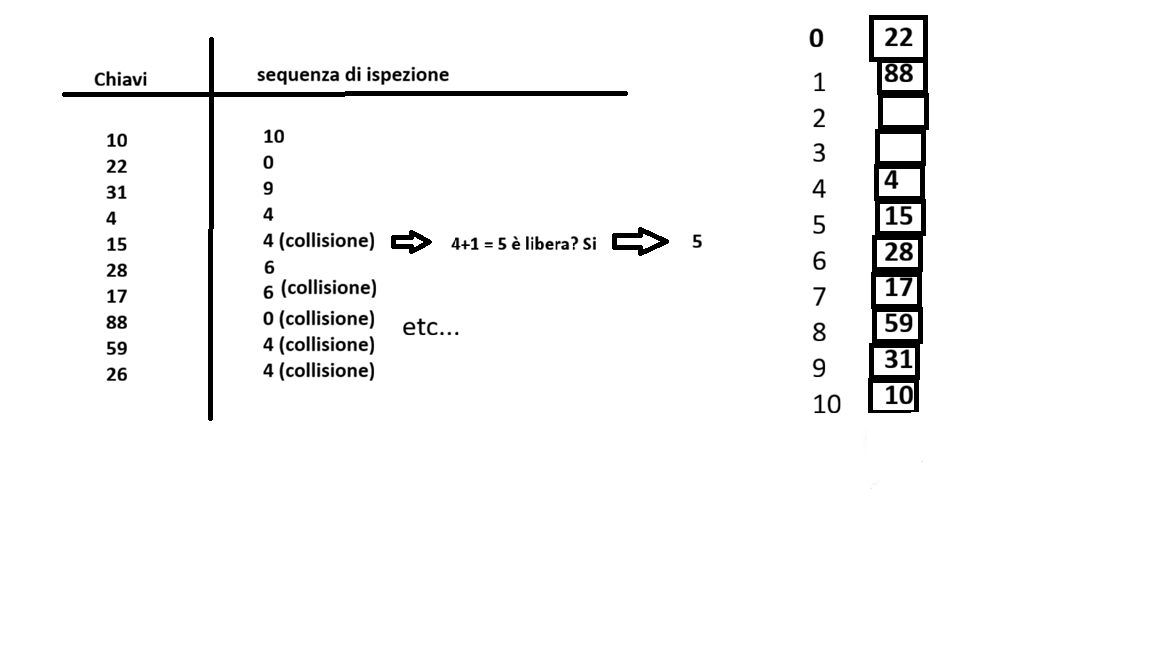
\includegraphics[width=0.9\textwidth]{images/HashTableExercise.png}
\end{figure}
\paragraph{Doppio Hash:} uno dei metodi migliori e con le migliori prestazioni, ho due funzioni hash ausiliarie $h_1$ e $h_2$.
\[
h(k,i) = (h_1(k) + i \cdot h_2(k)) mod m
\]
\begin{lstlisting}
    \\Ottimo: lineare, pessimo: n == m
    insert(T,k): \\senza cancellazioni
        i = 0
        repeat:
            j = h(k,i)
            if(T[j] == nul):
                T[j] = k
                return k
            else:
                i++
        until (i == m)
        throw Error(overflow tabella)

    \\Ottimo: lineare, pessimo: n == m
    search(T,k):
        i=0
        repeat:
            j = h(k,i)
            if(T[j] == k):
                return j
            i++
        until (T[j] == nul || i >= m)
        return nil

\end{lstlisting}

\section{Grafi}
I grafi sono un tipo di struttura dati e sono rappresentati da una coppia:
\[
G = (V,E)
\]
\[
V = nodi/vertici
\]
\[
E = archi (u,v): u,v \in V
\]
Esistono grafi:
\begin{itemize}
    \item \textbf{Orientati:} composti da coppie ordinate, un arco ha una direzione specifica, ha al massimo $n^2$ archi.
    \[(u,v) \ne (v,u)\]
    \item \textbf{Non orientati:} un arco è bidirezionale, ha al massimo $\frac{n(n+1)}{2}$ archi.
    \[
    (u,v) \equiv (v,u)
    \]
\end{itemize}
L'\textbf{ordine} di $G$ è il numero di vertici, ovvero $|V|$.\\
La \textbf{dimensione} di un grafo è:
\[
dim(G) = |V| + |E|
\]
Se $(u,v) \in E$ allora:
\begin{itemize}
    \item $u$ e $v$ sono \textbf{adiacenti} (o vicini).
    \item $(u,v)$ è \textbf{incidente} su $u$ e $v$.
    \item $\forall v$, il \textbf{grado} di $v$, indicato con $\delta(v)$, corrisponde al numero di archi incidenti su $v$.
    \item $v$ è \textbf{isolato} $\Leftrightarrow \delta(v) = 0$.
    \item $u \leadsto v$ è il \textbf{cammino} tra tali nodi ed è una sequenza di nodi a due a due adiacenti che parte da $u$ e finisce in $v$.
    \item Un cammino è un \textbf{ciclo} se torna al nodo di partenza.
    \item Un cammino è \textbf{semplice} se ha tutti nodi distinti e quindi non contiene cicli.
    \item $\delta(u,v)$ è la \textbf{distanza} tra due nodi, che corrisponde alla lunghezza del cammino minimo tra i due.
\end{itemize}
Un grafo può essere anche:
\begin{itemize}
    \item \textbf{Sparso:}
    \[
    |E| = O(n) 
    \]
    (al massimo n)
    \item \textbf{Denso:}
    \[
    |E| = \Theta(n^2)
    \]
    \item \textbf{Completo (o Clique / Cricca)}: ogni coppia di vertici distinti è adiacente, massimo numero di archi possibile.
    \item \textbf{Connesso:} se ogni coppia di nodi è connessa, ovvero esiste un cammino che li connette.
    \item \textbf{Aciclico(DAG):} è senza cicli.
\end{itemize}
Un grafo $G^| = (V^|,E^|)$ è \textbf{sottografo} di $G = (V,E)$ se:
\[
V^| \subseteq V
\]
\[
E^| \subseteq E
\]
Una \textbf{componente connessa} di un grafo è un sottografo massimale di tale grafo.\\\\
I grafi possono essere rappresentati come:
\begin{itemize}
    \item \textbf{Matrici di adiacenza:} le righe e le colonne rappresentano i nodi, le celle indicano se esiste l'arco tra quella coppia di nodi o meno e occasionalmente anche un \textbf{valore} se il grafo è \textbf{pesato}.
    \item \textbf{Liste di adiacenza:} rappresentato da una lista di liste, ogni indice della lista principale contiene una lista dei nodi a cui il nodo contenente la lista è collegato. La lista è $nul$ se il grado del nodo è $0$.
\end{itemize}

\subsection{Grafi non orientati}
Nei grafi non orientati vale questo lemma:
\[
\sum_{v \in V} \delta(v) = 2|E|
\]
\subsection{Grafi orientati}
Nei grafi orientati vale questo lemma:
\[
\sum_{v \in V} \delta(v) = |E|
\]
In questo tipo di grafo, i nodi hanno:
\begin{itemize}
    \item \textbf{Grado in entrata:} $\delta^+(u)$
    \item \textbf{Grado in uscita:} $\delta^-(u)$
\end{itemize}
Il grado di un nodo corrisponde alla somma di questi due.\\
Un grafo ordinato è \textbf{fortemente connesso} se ogni coppia di nodi è connessa.\\
La definizione è analoga per \textbf{componente fortemente connessa}.

\subsection{Complessita delle operazioni (Matrice di adiacenza)}
\begin{center}
\begin{tabular}{|l|c|c|c|}
\hline
Operazione & Grafo orientato & Grafo non orientato & Note\\
\hline
adiacenti(u,v) & $\Theta(1)$ & $\Theta(1)$ & return[u,v]\\
grado(n) & $\Theta(n)$ & $\Theta(n)$ & scansiono la riga $u$ di $M$\\
aggiungiArco(u,v) & $\Theta(1)$ & $\Theta(1)$ & M[u,v] = 1 (M[v,u] = 1)\\
rimuoviArco(u,v) & $\Theta(1)$ & $\Theta(1)$ & analogo con "0"\\
\hline
\end{tabular}
\end{center}

\subsection{Complessita delle operazioni (Liste di adiacenza)}
\begin{center}
\begin{tabular}{|l|c|c|c|}
\hline
Operazione & Grafo orientato & Grafo non orientato & Note\\
\hline
adiacenti(u,v) & $\Theta(\delta(u))$ & $\Theta(\delta^-(u))$ & find($adj(u),v$)\\
grado(n) & $\Theta(\delta(u))$ & $\Theta(\delta^-(u))$ & adj(u).size\\
aggiungiArco(u,v) & $\Theta(1)$ & $\Theta(1)$ & $\Theta(\delta(u))$ se liste ordinate\\
rimuoviArco(u,v) & $\Theta(\delta(u))$ & $\Theta(\delta(u) + \delta(v))$ &\\
\hline
\end{tabular}
\end{center}
Ovviamente per aggiungiArco con liste ordinate e grafo non orientato la complessità è $\Theta(\delta(u) + \delta(v))$.

\subsection{Visite sui grafi}
Una visita su un grafo è un esame sistematico di tutti i vertici e di tutti gli archi di un grafo. (Oppure limitatamente di vertici e archi raggiungibili da una sorgente).\\
\subsubsection{BFS}
La visita \textbf{BFS (Breadth First Search)}, ovvero la \textbf{visita in ampiezza}, se $s \in V$ è nodo sorgente allora:
\[
bfs(G,s)
\]
scopre tutti i vertici raggiungibili da $s$ in ordine crescente rispetto alla distanza da $s$. Questo algoritmo utilizza una coda e visita tutto il grafo solo se è connesso.\\
Vediamo un esempio, diciamo che:
\begin{itemize}
    \item $v.d =$ distanza da $s$ di $v$.
    \item $v.status =$ può essere "A" (da visitare), "B" (Visitato), "C" (Visitato e visitati tutti gli archi uscenti).
    \item $v.\pi =$ predecessore (vertice da cui si arriva in v)
\end{itemize}
\begin{lstlisting}
    forEach v do:
        v.d = +inf
        v.pi = nul
        v.status = A
    s.status = B
    s.d = 0
    s.pi = nul
    Q = nuovaCoda()
    Enqueue(Q,s)
    while(Q != empty) do:
        u = dequeue(Q)
        forEach v in adj[u] do:
            if(v.status == A):
                v.status = B
                v.pi = u
                v.d = u.d + 1
            Enqueue(Q,v)
        u.status = C
\end{lstlisting}
\paragraph{Spiegazione del codice:} si inizializza tutto come si deve, il nodo sorgente ovviamente non ha predecessori ed è il primo da visitare (primo nella coda).\\
Dopo, si visita ogni nodo adiacente del primo nodo e li mette in coda (non è specificato nessun ordine specifico). Una volta visitati tutti i vicini, il nodo iniziale viene segnato col grado C e viene tolto dalla coda.\\
Il nodo in testa adesso è il secondo della visita e si deve ripetere il procedimento.\\
\paragraph{Complessità:} $\Theta(|V| + |E|) = \Theta(n + m)$ \\
Vediamo adesso un metodo che stampa un percorso minimo dopo aver svolto una BFS:
\begin{lstlisting}
print-path(G,s,v):
    if(v == s):
        print "s"
        return
    if(v.pi == nul):
        "v non e raggiungibile"
    else:
        print-path(G,s,v.pi)
        print "v"
\end{lstlisting}
\paragraph{Complessità:} $\Theta(1)$ se il path non esiste, altrimenti $\Theta(d(s,v))$, ovvero la distanza tra i due nodi.\\\\
Dimostriamo adesso una proprietà della visita BFS tramite alcuni lemmi.
\paragraph{Proprietà:} la BFS calcola la distanza $\delta(s,v)$ di ogni nodo dalla sorgente e dopo l'esecuzione tale valore è salvato in $v.d$.\\
\paragraph{Lemma 1}
\[
G = (V,E), s \in V
\]
\[
\forall (u,v) \in E, d(s,v) \leq d(s,u) + 1
\]
Un cammino da $s$ a $v$ può esistere più breve di quello passando da $u$, ma se ne esistesse uno più lungo non verrebbe attribuito a $v.d$.
\paragraph{Lemma 2:} al termine di un BFS(G,s):
\[
\forall v \in V, v,d \geq d(s,v)
\]
\paragraph{Dimostrazione Lemma 2:} vediamo prima il caso base:
\[
s.d = 0 = \delta(s,s)
\]
\[
\forall v \in V \ne s, v.d = +\infty \geq d(s,v)
\]
Quindi dopo il primo Enqueue, tutti i nodi tranne $s$ hanno sempre la distanza settata a infinito.\\
Vediamo adesso il caso induttivo con l'ipotesi induttiva: $u.d \geq \delta(s,u)$ e sapendo che il nodo $v$ viene scoperto da $u$.
\[
v.d = u.d + 1 \geq \delta(s,u) + 1
\]
Questa sopra è l'ipotesi induttiva applicata a cosa avviene nel ramo "then".
\[
\delta(s,u) + 1 \geq \delta(s,v)
\]
Questo sopra è il Lemma 1, dimostrazione completata dato che questo valore non verrà più modificato.
\paragraph{Lemma 3:} dopo l'esecuzione di un BFS, se:
\[
Q = \{v_1,v_2,\ldots,v_r\}
\]
Allora:
\[
v_r.d \leq v_1.d + 1
\]
\[
v_i.d \leq v_{i+1}.d
\]
\[
\forall i = 1,\ldots,r-1
\]  
Ricordiamo che con $v_r$ si intende l'ultimo elemento della coda in uno specifico momento, non l'ultimo nodo in assoluto da visitare.\\
Tutto questo si può dimostrare dal concetto di BFS, ovvero il fatto che tale algoritmo procede a "livelli" e una volta superato un livello ne dimentica un altro.
\paragraph{Corollario 4:} anche questo serve a dimostrare la proprietà. I valori delle distanze da $s$ dei vertici inseriti nella Queue sono monotoni crescenti (debolmente crescenti o strettamente crescenti) e quindi:
\[
v_i.d \leq v_j.d
\]
Se $v_i$ viene inserito prima di $v_j$ nella Queue.
\paragraph{Teorema di correttezza di BFS:} ricapitolando, un BFS scopre tutti i vertici che sono raggiungibili da $s$ sorgente e alla fine della sua esecuzione si avverano queste cose:
\begin{enumerate}
    \item $\forall v \in V, v.d = \delta(s,v)$.
    \item $\forall v \ne s$, con $v$ raggiungibile da $s$, uno dei cammini minimi da $s$ a $v$ è un cammino minimo da $s$ a $v.\pi$ seguito da $(v.\pi,v)$.
\end{enumerate}
\paragraph{Dimostrazione per assurdo punto 1:} supponiamo che:
\[
\exists v : v.d \ne \delta(s,v)
\]
Dato il Lemma 2 però, viene implicato questo:
\[
v.d > \delta(s,v)
\]
Consideriamo anche che $\delta(s,v)$ sia la distanza minima tra quelle dei vertici che soddisfano la condizione assurda e che un nodo $u$ precede $v$ in un cammino minimo da $s$ a $v$ e quindi:
\[
\delta(s,v) = \delta(s,u) + 1
\]
Siccome abbiamo detto che $v$ è il primo "errore" che si incontra allora $u$ è corretto:
\[
u.d = \delta(s,u)
\]
A questo punto la BFS esplora i vicini di $u$ e quindi, se non è stato ancora visitato, anche $v$ e succede questo:
\[
v.d = u.d + 1 = \delta(s,u) + 1 = \delta(s,v)
\]
In un altro caso, $v$ non può essere gia stato scoperto perchè $v$ può essere scoperto solo da un nodo con distanza $\delta(s,v) - 1$, quindi proprio $u$, nessun altro. (Corollario 4)\\
Dimostrazione completata.
\subsubsection{DFS}
La \textbf{DFS (Depth First Search)} sceglie un $v \in V$ e visita tutta la porzione del grafo raggiungibile da $v$ seguendo percorsi il più \textbf{profondi} possibile e seguendo solo archi non ancora esplorati.\\
Ovviamente gli archi vengono visitati partendo dall'ultimo vertice visitato che contiene archi uscenti non visitati.\\
Prima di vedere il codice, stabiliamo che:
\begin{itemize}
    \item $v.d = $ (la d sta per discovery) registra il momento in cui si incontra $v$ per la prima volta.
    \item $v.F = $ (la F sta per fine visita) registra il momento in cui termina la visita di $v$ (visitati tutti gli elementi di adj(v))
    \item $v.\pi = $ predecessore del nodo
    \item $v.status =$ può essere "A" (da visitare), "B" (Visitato), "C" (Visitato e visitati tutti gli archi uscenti).
    \item time = variabile globale
\end{itemize}
\begin{lstlisting}
DFS(G):
    forall v in V do:
        v.status = A
        v.pi = nul
    time = 0
    forall v in V do:
        if(v.status == A):
            DFS-VISIT(G,v)

DFS-VISIT(G,u):
    time++
    u.d = time
    u.status = B
    forall v in adj(u) do:
        if(v.status == A):
            v.pi = u
            DFS-VISIT(G,v)
    u.status = C
    time++
    u.f = time
\end{lstlisting}
\paragraph{Spiegazione del codice:} si svolge la visita DFS per ogni sorgente, dato che un grafo può avere componenti connesse distinte.
\paragraph{Complessita:} $\sum_{u \in V}^{\delta(u)} = |E| = m$.\\
Ogni sottografo generato dalla DFS è detta \textbf{Foresta DFS}.\\
\paragraph{Teorema delle parentesi:} se $u,v \in V$ e $I_u = [u.d,u.f]$ e $I_v = [v.d,v.f]$ allora sono una di queste è vera:
\begin{itemize}
    \item $I_u \cap I_v = \emptyset$ (i nodi sono distinti e nessuno è discendente dell'altro.) (un discendente di un nodo fa parte dei suoi adiacenti)
    \item $I_u \subset I_v$ (u è discendente di v)
    \item $I_v \subset I_u$ (v è discendente di u)
\end{itemize}
\paragraph{Classificazione degli archi su grafi orientati:}
\begin{itemize}
    \item \textbf{Archi d'albero:} $(u,v) \in E$ è un arco d'albero se $u = v.\pi$ (v è A quando si ispeziona)
    \item \textbf{Archi all'indietro:} se $v$ è antenato di $u$ (v è B quando si ispeziona)
    \item \textbf{Archi in avanti:} archi che non sono d'albero e v è discendente di u (v è C quando viene ispezionato)
    \item \textbf{Archi trasversali:} se u e v non sono discendenti uno dell'altro.
    \item 
\end{itemize}
\paragraph{Teorema del cammino bianco:} v è discendente di u se e solo se, al momento in cui u viene scoperto (u.d), esiste un cammino di soli nodi bianchi da u a v.\\
\paragraph{Dimostrazione:}
\begin{itemize}
    \item $u == v \implies$ il cammino è formato solo da u che è bianco al momento.
    \item $u \ne u \implies$ se v è discendente di u allora il suo intervallo è sottoinsieme dell'intervallo di u. Siccome v viene scoperto dopo u, è bianco all'istante u.d (v.d > u.d).
\end{itemize}
\paragraph{Classificazione degli archi su grafi non orientati}
In questo caso gli archi possono essere solo d'albero o all'indietro.\\
Ogni arco viene ispezionato due volte e la classificazione si fa la prima volta che si analizza.\\
\paragraph{Dimostrazione:}
\begin{itemize}
    \item Caso 1: $(u,v)$ esplorato la prima volta da u verso v, in questo caso v è A e l'arco è d'albero.
    \item Caso 2: $(u,v)$ esplorato la prima volta da v verso u, in tal caso è all'indietro.
\end{itemize}
\paragraph{Teorema:} un grafo è ciclico se e solo se contiene un arco all'indietro.\\
\paragraph{Dimostrazione:} la definizione di un arco $(u,v)$ all'indietro dice che $u$ è antenato di $v$ e quindi da $u$ si può raggiungere $v$. Se uniamo il cammino da $u$ a $v$ con l'arco all'indietro $(v,u)$ allora si forma un ciclo.\\
Inoltre, gli archi di un ciclo non possono essere tutti d'albero, ce ne deve essere almeno uno all'indietro.\\
Se il grafo invece è orientato supponiamo che v sia il primo vertice di un ciclo ad essere scoperto e diventare grigio, gli altri vertici sul ciclo al momento sono bianchi.\\
Sia u il vertice che precede v, tutti i vertici sul cammino da v a u sono bianchi e per il teorema del cammino bianco u è discendente di v e quindi v è antenato di u e $(u,v)$ è un arco all'indietro.
\subsubsection{Ordinamento topologico e DAG}
Un \textbf{DAG} è un \textbf{Directed Acyclic Graph}, ovvero un grafo direzionato aciclico.\\
Un algoritmo per un ordinamento topologico prende in input un DAG e ritorna appunto un ordinamento topologico, ovvero una sequenza di nodi di $G$ tale che:
\[
\forall (u,v) \in E, u \text{ precede } v
\]
L'ordinamento topologico di un DAG non è unico.\\
Può essere applicato per stabilire un ordine di eventi.\\
\begin{lstlisting}
OT(G):
    DFS(G) //ma aggiungo in testa a L u quando faccio u.f = k
    return L
\end{lstlisting}
Ha complessita quanto una DFS più gli inserimenti in L:
\[
\Theta(n+m) + \Theta(n) = \Theta(n+m)
\]
\paragraph{Teorema di correttezza dell'OT:} l'algoritmo di OT(G) produce un ordinamento topologico del DAG G.
\paragraph{Lemma 1:} G è un DAG $\Leftrightarrow$ DFS(G) non ha archi all'indietro. (e quindi non ci sono cicli, già dimostrato secondo un teorema sopra)
\subsection{Algoritmo di Dijkstra}
Il problema che risolve l'\textbf{algoritmo di Dijkstra} è questo:\\
"Data un'origine u e una destinazione v in un grafo orientato pesato con pesi non negativi, determinare il percorso più conveniente da seguire".\\
Con "conveniente" spesso si intende il più efficiente, per esempio nei grafi con archi pesati, come per esempio l'instradamento di pacchetti (routing) o la ricerca del miglior percorso stradale su Google Maps.\\
Intuitivamente, in un grafo non pesato il cammino minimo da u a v è proprio quello con il minimo numero di archi e si trova:
\begin{itemize}
    \item BFS(G,u)
    \item Percorso da u a v seguendo gli archi $pi$.
\end{itemize}
Per i grafi pesati invece stabiliamo:
\[
G = (V,E)
\]
\[
\omega: E \to \mathbb{R}
\]
Quest'ultima è una \textbf{funzione peso}.\\
Tale funzione può calcolare anche il peso di un cammino:\\
\[
p = <v_0,\ldots,v_k>
\]
\[
\omega(p) = \omega(v_0,v_1) + \omega(v_1,v_2) + \cdots + \omega(v_{k-1},v_k) = \sum_{i = 1}^{k} \omega(v_{i-1},v_i)
\]
Il peso di un cammino minimo è tale omega se esso esiste, infinito altrimenti.
\subsubsection{Variante dei cammini con sorgente unica}
Mettiamo caso che $s \in V$ sia una sorgente del grafo e bisogna calcolare il cammino di peso minimo da $s$ a ogni $v \in V$.\\
\begin{itemize}
    \item Si può invertire il problema, riconducendosi a cammini minimi con destinazione unica (ovvero la sorgente)
    \item Si può sostituire s con u se il problema chiede di calcolare il cammino minimo da u a v fissati.
    \item Se invece il problema ci chiede di calcolare il cammino minimo tra ogni coppia di nodi del grafo, basta sostituire la sorgente con ogni nodo e riusare sempre l'algoritmo per i cammini minimi.
\end{itemize}
\subsubsection{Proprietà dei cammini minimi}
\paragraph{Sottostruttura ottima:} i sotto-cammini di cammini minimi sono cammini minimi di sotto-problemi.
\paragraph{Lemma 1:} dato un grafo orientato $G  = (V,E)$ con la sua funzione peso $\omega : E \to \mathbb{R}$, sia $p = <v_1,\ldots,v_k>$ un cammino minimo da $v_1$ a $v_k$ e per qualsiasi $i$ e $j$ tali che $1 \leq i \leq j \leq k$ sia $P_{ij} = <v_i,\ldots,v_j>$ il sottocammino di p da $v_i$ a $v_j$, allora:
\begin{center}
    $p_{ij}$ è un cammino minimo da $v_i$ a $v_j$
\end{center}
\paragraph{Dimostrazione Lemma 1:} se appunto:
\[
\omega(p) = \omega(p_{1i}) + \omega(p_{ij}) + \omega(p_{jk})
\]
Supponiamo per assurdo che esista:
\[
p^|_{ij} : \omega(p^|_{1i}) < \omega(p_{ij})
\]
Questo significa che possiamo costruire un cammino $p^|$ tale che:
\[
\omega(p^|) = \omega(p_{1i}) + \omega(p^|_{ij}) + \omega(p_{jk}) < \omega(p)
\]
Questo però è falso per via della minimalità di $p$.\\\\
Se tutti i pesi nel grafo sono non negativi, allora:
\begin{itemize}
    \item Tutti i cammini minimi sono semplici, ovvero non contengono cicli, in quanto aggiungerebbe solo peso, se ci fossero pesi negativi al contrario potrebbe essere vantaggioso fare un ciclo.
    \item Ogni cammino contiene al massimo $|V|$ vertici e quindi $|V| - 1$ archi.
\end{itemize}
\subsubsection{Funzionamento dell'algoritmo di Dijkstra}
L'algoritmo, per ogni vertice, mantiene:
\begin{itemize}
    \item $v.\pi$ = predecessore (rispetto al cammino minimo)
    \item $v.d$ = stima del cammino minimo, limite superiore per il peso di un cammino minimo, è inizializzato a $\infty$
\end{itemize}
Tutti i vertici sono inseriti in una \textbf{coda PQ di Min-priorità} (con priorità $v.d$)\\
L'algoritmo seleziona ripetutamente il vertice $u$ con la minor priorità / stima del cammino minimo (estraendolo da PQ) ed esamina gli archi uscenti da u.\\
Per ogni vertice $v \in ADJ(u)$ controlla se passando da u si trova un cammino $s \to v$ meno costoso.\\
In tal caso, aggiorna $v.\pi$ e $v.d$ ("rilassamento" dell'arco $(u,v)$).
\begin{lstlisting}
DIJKSTRA(G,w (funzione peso),s (sorgente)):
    PQ = []
    s.d = 0
    s.pi = nul
    INSERT(PQ, s) //con proprita s.d
    for all v in V \ {s}:
        v.d = inf
        v.pi = nul
        INSERT(PQ, v)
    while (PQ != emptyset):
        u = EXTRACT-MIN(PQ)
        for all v in ADJ(u):
            dnew = u.d + w(u,v)
            if(dnew > v.d):
                v.d = dnew
                v.pi = u
                DECREASE-KEY(PQ, v, dnew)

\end{lstlisting}
La complessità di questo algoritmo è:
\[
O(|V| \cdot costo(EXTRACT-MIN) + |E| \cdot costo(DECREASE-KEY))
\]
\begin{itemize}
    \item Si eseguono $|V|$ operazioni $EXTRACT-MIN$
    \item La lista di adiacenza di ciascun vertice viene esaminata esattamente una volta.
    \item Ci sono in totale $|E|$ iterazioni del ciclo for (quello delle adiacenze) e quindi al più $|E|$ chiamate di DECREASE-KEY
\end{itemize}
In realtà esisterebbe anche un altro $+ \Theta(|V|)$ per l'inizializzazione, ma si omette.\\\\
Si può vedere che la complessita dipende da come è implementata la PQ, vediamo assieme i vari casi:
\paragraph{PQ è un array:}
\begin{itemize}
    \item Le operazioni INSERT e DECREASE-KEY hanno costo costante.
    \item EXTRACT-MIN ha costo $O(|V|)$ (occorre ispezionare tutto l'array per trovare un minimo)
    \item Il costo complessivo è $\Theta(|V|) + O(|V|^2 + |E|) = O(|V|^2)$
\end{itemize}
\paragraph{PQ è un MIN-heap binario:}
\begin{itemize}
    \item L'inizializzazione costa $\Theta(|V|)$
    \item EXTRACT-MIN costa $O(log|V|)$
    \item DECREASE-KEY costa $O(log|V|)$
    \item Costo complessivo è $\Theta(|V|) + O(|V|log|V| + |E|log|V|) = O((|V| + |E|)log|V|)$
\end{itemize}

\subsubsection{Teorema di correttezza}
Una volta che l'algoritmo è terminato:
\[
\forall v \in V : v.d = \delta(s,v)
\]
Ricordiamo che tale $\delta(s,v)$ è la lunghezza del cammino minimo tra s e v.\\
\paragraph{Dimostrazione per induzione:}
\begin{itemize}
    \item Se $v = s$ allora $s.d = 0 = \delta(s,s)$
    \item Se $v \ne s$ allora supponiamo che P sia un cammino minimo $(s,v)$ e che $(x,y) \in E$ sia il primo arco del cammino P dopo che si esce da $(s,x)$. Inoltre, x è gia stato aggiunto al cammino minimo mentre y è ancora in PQ.\\
    Adesso osserviamo che quando x è stato estratto l'arco $(x,y)$ è stato rilassato e quindi:
    \[
    y.d \leq x.d è \omega(x,y) = \delta(s,x) + \omega(x,y) = \omega(s,y)
    \]
    Dato che è minore o uguale alla lunghezza del cammino minimo e data la definizione di cammino "minimo" allora:
    \[
    y.d = \delta(s.v)
    \]
\end{itemize}



\section{Calcolabilità}
La \textbf{calcolabilità} si occupa delle questioni fondamentali circa la potenza e le limitazioni dei sistemi di calcolo.\\
Nacque nella prima metà del ventesimo secolo quando si scoprì l'esistenza dei problemi \textbf{non decidibili}, ovvero senza algoritmo risolutivo.\\
I problemi decidibili si suddividono in:
\begin{itemize}
    \item Trattabili (costo polinomiale)
    \item Intrattabili (costo esponenziale)
\end{itemize}
La calcolabilità classifica gli algoritmi in decidibili e non.\\
\subsection{Esistenza dei problemi indecidibili}
Due insiemi A e B hanno lo stesson numero di elementi se e solo se esiste una biiezione tra di loro.\\
Inoltre, cerchiamo di enumerare ogni possibile sequenza costruita su un alfabeto finito.\\
Si stabilisce un ordine tra i caratteri dell'alfabeto e, a pari lunghezza, in ordine alfabetico, in tal modo si da un ordine a tutto e sapremo quanti passi ci vorranno per raggiungere tale stato.\\
Ad una sequenza corrisponde quindi il suo numero di passi per raggiungerla.\\
Non è possibile enumerare le sequenze di lunghezza infinita.\\
Un \textbf{problema computazionale} può essere visto come una funzione matematica che associa ad ogni insieme di dati, espressi da $k$ numeri interi, il corrispondente risultato, indicato da $j$.\\
\[
f: N^k \to N^j
\]
Qualsiasi sia l'enumerazione di tali funzioni, questo insieme non è numerabile.\\\\
L'insieme degli algoritmi è numerabile e:
\[
Algoritmi << Problemi
\]
In quanto esistono problemi non risolvibili tramite algoritmo.\\
Un algoritmo dipende dal linguaggio utilizzato e consiste da una sequenza finita di operazioni.\\
Per quanto infiniti possano essere gli algoritmi, essi sono numerabili.\\
\subsection{Il problema dell'arresto}
Non è facile trovare un algoritmo non calcolabile.\\
Il problema dell'arresto è in forma decisionale:
\[
Arresto: \{Istanze\} \to \{0,1\}
\]
Preso un algoritmo A e dati di input D, decidere in tempo finito se l'esecuzione di A su D termina o no, quindi con A in input:
\[
Arresto(A,D) \to \{0,1\}
\]
Turing, ideatore di tale problema, riuscì a dimostrare che se un programma arbitrario si arresta e termina la sua esecuzione è una cosa impossibile e quindi è indecidibile.\\
Questo è dimostrabile dal fatto che, se A non terminasse allora ARRESTO non ritornerebbe mai tale informazione.\\
Quindi non può esistere un algoritmo che decida in tempo finito se un algoritmo arbitrario termina la sua esecuzione.\\
Ci sono moltissimi altri esempi:
\begin{itemize}
    \item L'algoritmo per trovare l'equivalenza tra due programmi è indecidibile (se per ogni possibile input, producono lo stesso output)
    \item L'algoritmo che determina se un programma è un malware è indecidibile (ovvero se compie azioni malevoli)
    \item Il decimo problema di Hilbert è indecidibile (determinare se una soluzione polinomiale con coefficienti interi ha soluzioni intere (equazioni diofantee))
\end{itemize}
\paragraph{Algoritmo di GOLDBACH:} restituisce il primo numero intero pari che non è risultato di una somma di due numeri primi qualsiasi.
\subsection{Tesi di Church-Turing}
Ogni modello di calcolo risolve esattamente la stessa classe di problemi, dunque si equivalgono nella possibilità di risolverli, pur avendo diversa efficienza.\\
Eventuali migliorie hardware o software servono solo a migliorare l'efficienza.
\subsection{Problemi trattabili e intrattabili}
Il problema della torre di Hanoi è intrattabile (cerca su internet).\\
Un altro algoritmo non trattabile è quello che calcola ogni possibile permutazione$G$ contiene una \textbf{clique} (cricca) di almeno $k$ nodi.\\
Un algoritmo per risolverlo è quello che considera tutti i sottinsiemi di vertici, in ordine decrescente di cardinalità, e verifica se formano una cricca di ordine k.\\
Tale algoritmo non è ancora stato trovato e si sospetta che non esista.\\
\paragraph{Cammino hamiltoniano:} cammino semplice che passa da tutti i vertici di G una volta sola.
\paragraph{Ciclo hamiltoniano:} cammino hamiltoniano chiuso.
Date queste due definizioni, un algoritmo per trovare un cammino hamiltoniano in un grafo non è noto, dovrebbe considerare tutte le permutazioni di vertici e verificare se sono consecutivi (a due a due adiacenti).

\section{Complessità}
\subsection{Differenza di potenza tra calcolatori}
Alcuni calcolatori sono più veloci di altri, per esempio se $C_2$ è $k$ volte più veloce di $C_1$, allora usare $C_2$ per un tempo $t$ equivale ad usare $C_1$ per un tempo $k \cdot t$.
\subsection{Categorizzazione dei problemi}
La categorizzazione dei problemi è in base alla domanda che ci facciamo:
\begin{itemize}
    \item \textbf{Problema decisionale:} ci si chiede se vale o meno una certa proprietà. (isAbr)
    \item \textbf{Problema di ricerca:} ricercare un qualcosa o restituire un oggetto dato un input. (ritorno di un cammino da un grafo)
    \item \textbf{Problema di ottimizzazione:} si vuole trovare la migliore soluzione tra tutte le soluzioni possibili. (Algoritmi Greedy)
\end{itemize}
Molta della teoria della complessita in questa sezione è definita principalmente in termini dei problemi di decisione.\\
Questo perchè non ci si deve preoccupare del tempo di formulazione dell'output, in quanto è soltanto un boolean. Inoltre, la complessita di ogni problema è riconducibile alla complessita del suo relativo problema decisionale.\\
Per esempio, un problema di ottimizzazione può essere definito come problema decisionale:
\begin{itemize}
    \item Problema di ottimizzazione: voglio trovare la clique più grande in un grafo G
    \item Problema decisionale associato: esiste una clique in G con almeno k vertici?
\end{itemize}
Il problema decisionale non è più difficile del problema di ottimizzazione: se sappiamo risolvere il problema di ottimizzazione, confrontiamo il risultato con k e quindi risolveremmo il problema decisionale di conseguenza.\\
Si può dire quindi che la complessita del problema di ottimizzazione ha un limite inferiore pari alla complessita del problema decisionale annesso.
\subsection{Time e Space}
\paragraph{Time(f(n)):} insiemi dei problemi decisionali che possono essere risolti in tempo O(f(n))
\paragraph{Space(f(n)):} insiemi dei problemi decisionali che possono essere risolti in spazio O(f(n))
\subsection{Classi di problemi}
\begin{itemize}
    \item \textbf{classe P} è la classe dei problemi risolvibili in tempo polinomiale nella dimensione n dell'istanza di ingresso.
    \item \textbf{classe PSPACE:} è la classe dei problemi risolvibili in spazio polinomiale nella dimensione n dell'istanza di ingresso.
    \item \textbf{Classe EXP Time:} è la classe dei problemi risolvibili in tempo esponenziale nella dimensione n dell'istanza di ingresso.
\end{itemize}
Inoltre:
\[
P \subseteq PSPACE
\]
\[
PSPACE \subseteq ExpTime \implies P \subseteq ExpTime
\]
Problemi in tempo esponenziale:
\begin{itemize}
    \item Commesso Viaggiatore
    \item Clique
    \item Cammino hamiltoniano
    \item Soddisfacibilità di formule booleane (SAT)
    \item Torre di Hanoi
\end{itemize}
\subsubsection{SAT}
Insieme V di variabili booleane:
\begin{itemize}
    \item Letterale: variabile o sua negazione
    \item Clausola: disgiunzione (OR) di letterali
\end{itemize}
Un espressione booleana su V si dice in \textbf{forma normale congiuntiva (FNC)} se è espressa come \textbf{congiunzione di clausole} (AND di OR letterali)\\
Per i SAT si considerano tutti i $2^n$ assegnamenti possibili (possibili combinazioni) su $n$ variabili in input e si controlla se risulta vero il risultato o meno. Questo algoritmo non è noto in quanto non si sa se è risolvibile in tempo polinomiale e quindi si presume sia esponenziale (Tutti gli SAT).
\subsection{Certificati}
In un problema decisionale siamo interessati a verificare se un istanza del problema soddisfa una certa proprietà, ovvero saper rispondere ad una domanda per una qualsiasi istanza in input.\\
Per alcuni problemi, per le \textbf{istanze accettabili} (Un input specifico accettabile) è possibile fornire un \textbf{certificato}, ovvero un \textbf{attestato breve di esistenza} di una soluzione ad un dato problema.\\
Un certificato di non esistenza è facile da costruire ma sicuramente non breve.\\
Vediamo un esempio di applicazione dove si applica il costo del certificato per determinare il costo del problema generale:\\
PI è un problema in tempo polinomiale se:
\begin{itemize}
    \item Ogni istanza accettabile nel problema (ogni possibile input) di lunghezza n ammette un certificato y di lunghezza polinomiale in n
    \item Esiste un algoritmo di verifica polinomiale in n e applicabile a ogni coppia <x,y> che permette di attestare che l'input è accettabile
\end{itemize}
La \textbf{classe NP} è la classe dei problemi decisionali verificabili in tempo polinomiale (NON polinomiali). Questa classe è l'insieme dei problemi risolvibili in tempo polinomiale non deterministico.\\
\[
P \subseteq NP
\]
Ogni problema P ammette un certificato verificabile in tempo polinomiale, basta seguire l'algoritmo che risolve il problema per costruire il certificato.\\
In realtà non si sa se:
\[
P = NP
\]
o se:
\[
P \ne NP
\]
Si è certi che siano diversi, ma nessuno sa dimostrarlo.\\
Ma è possibile individuare i problemi più difficili all'interno della classe NP, ovvero quelli che sono in NP / P se P fosse diverso da NP, sono i problemi \textbf{NP-Completi}.\\
Tali problemi sono quelli provatamente più difficili della classe NP\\
Se esistesse un algoritmo polinomiale in grado di risolvere uno di questi problemi allora tutti tali problemi lo sarebbero e quindi:
\[
P = NP
\]
Se invece si potesse dimostrare che almeno uno di questi problemi non offre un algoritmo risolutivo polinomiale allora:
\[
P \ne NP
\]
In realtà, o li risolvo tutti in tempo polinomiale, o non ne risolvo nessuno.
\subsubsection{Riduzione polinomiale}
Presi due problemi A e B decisionali e $I_1$ e $I_2$ insiemi delle istanze dei due problemi, A si riduce in tempo polinomiale a B:
\[
A \leq_p B
\]
Se esiste una funzione $f:I_1 \to I_2$ calcolabile in tempo polinomiale tale che per ogni istanza x di A:
\begin{itemize}
    \item x è istanza accettabile di A SE E SOLO SE f(x) lo è di B
\end{itemize}
Questo implica che se esiste un algoritmo polinomiale per risolvere B, allora esiste anche per risolvere A, ci si può ricondurre ad un problema più piccolo(?) e risolvere quello, quindi l'input viene prima tramutato in input di un problema secondario e poi viene risolto il problema secondario, questo equivale a risolvere il primo problema.\\
Un problema decisionale C si dice NP-completo se:
\begin{itemize}
    \item $C in NP$
    \item $\forall C^| \in NP, C^| \leq_p C$
\end{itemize}
Un problema C si dice \textbf{NP-Arduo} se:
\[
\forall C^| \in NP, C^| \leq_p C
\]
Quindi C non è necessariamente in NP.
\subsubsection{Teorema di Cook (1971)}
Ha dimostrato che ogni SAT è NP-Completo.\\
Un problema A decisionale si dice NP-Completo se:
\begin{itemize}
    \item $A \in NP$
    \item $SAT \leq_p A$
\end{itemize}
Per esempio, Clique è completo: per ogni clausola di SAT si tramutano i propri elementi in vertici:\\
SAT = (a OR b) AND (c OR d) AND !a\\
Vertici = (a,b,c,d,!a)\\
Gli archi invece si connette ogni elemento di ogni clausola con elementi che:
\begin{itemize}
    \item Non sono della stessa clausola
    \item Sono diversi dal negativo del vertice a cui collegarsi (per esempio a non verrà collegato con !a)
\end{itemize}
Archi = ((a,c),(a,d),(b,c)(b,d)(b,!a)(c,!a)(d,!a))\\
In tale grafo esiste una cricca se SAT è soddisfacibile, infatti ogni cricca contiene elementi tutti di clausole diverse e la loro combinazione risolve la formula (ritornando vero per SAT).\\
Questo vale anche al contrario, se SAT è soddisfacibile allora esiste una clique in G.\\\\
I problemi \textbf{NP equivalenti} sono problemi che tra di loro sono appunto equivalenti...\\
Per esempio, SAT e clique sono tra di loro equivalenti, ma anche tutti gli NP-Completi lo sono tra di loro.\\
\paragraph{Altri prolemi importanti:}
\begin{itemize}
    \item Vertex cover per grafi
    \item Graph Coloring (colorare con più k colori possibili tale che due vertici adiacenti non abbiano mai lo stesso colore), questo è per esempio connesso alla colorazione della cartina politica (divisione degli stati) del mondo.
\end{itemize}
\subsection{Esercizi}
\subsubsection{Come risolvere esercizi}
Se ti chiedono di controllare se la versione decisionale di un problema è in NP allora devi:
\begin{itemize}
    \item Capire il problema iniziale
    \item Individuare il problema decisionale associato
    \item Trovare un certificato
    \item Trovare l'algoritmo che controlla il certificato
    \begin{itemize}
        \item In questo, prima si controlla che il certificato sia del formato giusto
        \item Poi si controlla che il certificato sia valido o meno
        \item Si calcola la complessita dell'algoritmo e si traggono le conclusioni.
    \end{itemize}
\end{itemize}
Se invece ti chiedono di trasformare una SAT in una clique, sai gia come fare dalle sezioni precedenti.
\subsubsection{Problema 1}
Eseguire la riduzione polinomiale da SAT a Clique per:
\[
F = (x \lor y) \land (!x \lor z) \land y \land z
\]
Mostrando la k-clique e il relativo assegnamento positivo.\\
Costruiamo il grafo intanto:
\[
Vertici = [x, y, !x, z, y_2, z_2]
\]
\[
Archi = [(x,z),(x,y_2),(x,z_2),(y,!x),(y,z),(y,y_2),(y,z_2),(!x,y),(!x,y_2),(!x,z_2),(z,x),(z,y),(z,y_2),(z,z_2),(y_2,x),(y_2,y),(y_2,!x),(y_2,z),(y_2,z_2),(z_2,x),(z_2,y),(z_2, !x),(z_2,z)]
\]
La clique massima è di 4 nodi e ne esistono 2:
\begin{itemize}
    \item x = false, y = true, z = true
    \item y = true, z = true
\end{itemize}
\subsubsection{Problema 2}
G = (V,E) dove per ogni $u \in V$ voglio assegnare $C[u]$ colore. Dimostrare che la versione decisionale del problema 3-colorazione è in NP.\\
Per ricordarsi, tale problema chiede se è possibile colorare ogni nodo con un massimo 3 colori in modo che due nodi adiacenti non siano mai dello stesso colore.\\
Bisogna esibire un certificato C e una verifica di costo polinomiale.\\
\begin{lstlisting}
verifica3color(G,C[]): \\C = insieme di assegnazioni vertice-colore
    D = array di n elementi
    for i=1 to n do:
        D[i] = C[i] \\copio C in D
    sort(D)
    d = 1 \\contatore di colori
    for i=2 to n do:
        if (d[i] != d[i-1]):
            d++
    if(d > 3):
        return false
    forall u in V do:
        forall v in ADJ[u] do:
            if(C[u] == C[v]):
                return false
    return true
\end{lstlisting}
Questo codice controlla se il certificato è valido.\\
Per capire se rientra in NP, rimane da controllare che la complessita sia polinomiale:
\begin{itemize}
    \item $\Theta(n)$ per la copia dell'array
    \item $\Theta(n \cdot log(n))$ per il sort (Merge Sort)
    \item $\Theta(n)$ per il conteggio dei colori (confronto solo con l'elemento prima perche ho usato sort)
    \item $\Theta(n \cdot |adj[u]|)$ scorro tutti i vicini di tutti i nodi e quindi $ = \Theta(|E|) = \Theta(m)$
\end{itemize}
Quindi la complessità è $\Theta(n + m)$, che è polinomiale. Si può dire che tale problema è in NP.

\subsubsection{Problema 3}
La versione decisionale del problema dello zaino 0-1 è in NP?\\
Sappiamo che abbiamo:
\[
W = peso massimo da portare
\]
\[
V = valore minimo da portare
\]
\[
v[] = valori dei vari oggetti
\]
\[
w[] = peso dei vari oggetti
\]
Ci serve un certificato e un algoritmo che lo controlli in tempo polinomiale.\\
\textbf{Certificato:}
Un vettore binario $C[1..n]$ tale che:
\[
C[i] =
\begin{cases}
1 & \text{se l'oggetto } i \text{ è scelto} \\
0 & \text{altrimenti}
\end{cases}
\]
\textbf{Verificatore:}
\begin{lstlisting}
verificaZaino(w[],v[],V,W,C[]):
    for i=1 to n do:
        if(C[i] != 0 AND C[i] != 1):
            return false \\certificato errato
    p = 0 \\peso totale
    val = 0 \\valore totale
    for i=1 to n do:
        if(C[i] == 1):
            p += w[C[i]]
            val += v[C[i]]
    if(val < V): return false
    if(p > W): return false
    return true
\end{lstlisting}
\textbf{Complessità:}
Il verificatore esegue un singolo ciclo sugli $n$ oggetti, quindi ha complessità $O(n)$.

\section{Altri algoritmi}
\subsection{Array non ordinato}

\subsubsection{Ricerca}
Scansione lineare sequenziale fino a trovare l’elemento.
\begin{itemize}
    \item Caso migliore: $O(1)$
    \item Caso medio: $O(n)$
    \item Caso peggiore: $O(n)$
\end{itemize}

\subsubsection{Inserimento}
Inserimento in ultima posizione (se c’è spazio disponibile).
\begin{itemize}
    \item Caso migliore: $O(1)$
    \item Caso medio: $O(1)$
    \item Caso peggiore: $O(1)$ (oppure $O(n)$ se serve ridimensionamento)
\end{itemize}

\subsubsection{Cancellazione}
Ricerca dell’elemento e sostituzione con l’ultimo elemento.
\begin{itemize}
    \item Caso migliore: $O(1)$
    \item Caso medio: $O(n)$
    \item Caso peggiore: $O(n)$
\end{itemize}


\subsection{Array ordinato}

\subsubsection{Ricerca}
Ricerca binaria.
\begin{itemize}
    \item Caso migliore: $O(1)$
    \item Caso medio: $O(\log n)$
    \item Caso peggiore: $O(\log n)$
\end{itemize}

\subsubsection{Inserimento}
Ricerca binaria per trovare la posizione + shift degli elementi successivi.
\begin{itemize}
    \item Caso migliore: $O(n)$
    \item Caso medio: $O(n)$
    \item Caso peggiore: $O(n)$
\end{itemize}

\subsubsection{Cancellazione}
Ricerca binaria + shift degli elementi successivi.
\begin{itemize}
    \item Caso migliore: $O(n)$
    \item Caso medio: $O(n)$
    \item Caso peggiore: $O(n)$
\end{itemize}


\subsection{Lista non ordinata (semplicemente concatenata)}

\subsubsection{Ricerca}
Scansione lineare nodo per nodo.
\begin{itemize}
    \item Caso migliore: $O(1)$
    \item Caso medio: $O(n)$
    \item Caso peggiore: $O(n)$
\end{itemize}

\subsubsection{Inserimento}
Inserimento in testa.
\begin{itemize}
    \item Caso migliore: $O(1)$
    \item Caso medio: $O(1)$
    \item Caso peggiore: $O(1)$
\end{itemize}

\subsubsection{Cancellazione}
Ricerca del nodo precedente + aggiornamento dei puntatori.
\begin{itemize}
    \item Caso migliore: $O(1)$
    \item Caso medio: $O(n)$
    \item Caso peggiore: $O(n)$
\end{itemize}


\subsection{Lista ordinata (semplicemente concatenata)}

\subsubsection{Ricerca}
Scansione lineare fino al valore o superamento.
\begin{itemize}
    \item Caso migliore: $O(1)$
    \item Caso medio: $O(n)$
    \item Caso peggiore: $O(n)$
\end{itemize}

\subsubsection{Inserimento}
Ricerca posizione corretta + aggiornamento puntatori.
\begin{itemize}
    \item Caso migliore: $O(1)$
    \item Caso medio: $O(n)$
    \item Caso peggiore: $O(n)$
\end{itemize}

\subsubsection{Cancellazione}
Ricerca nodo + aggiornamento puntatori.
\begin{itemize}
    \item Caso migliore: $O(1)$
    \item Caso medio: $O(n)$
    \item Caso peggiore: $O(n)$
\end{itemize}


\subsection{Lista doppia non ordinata}

\subsubsection{Ricerca}
Scansione lineare (in avanti o bidirezionale).
\begin{itemize}
    \item Caso migliore: $O(1)$
    \item Caso medio: $O(n)$
    \item Caso peggiore: $O(n)$
\end{itemize}

\subsubsection{Inserimento}
Inserimento in testa (aggiornamento di due puntatori).
\begin{itemize}
    \item Caso migliore: $O(1)$
    \item Caso medio: $O(1)$
    \item Caso peggiore: $O(1)$
\end{itemize}

\subsubsection{Cancellazione}
Ricerca nodo + aggiornamento di entrambi i puntatori.
\begin{itemize}
    \item Caso migliore: $O(1)$
    \item Caso medio: $O(n)$
    \item Caso peggiore: $O(n)$
\end{itemize}


\subsection{Lista doppia ordinata}

\subsubsection{Ricerca}
Scansione lineare fino al valore o superamento.
\begin{itemize}
    \item Caso migliore: $O(1)$
    \item Caso medio: $O(n)$
    \item Caso peggiore: $O(n)$
\end{itemize}

\subsubsection{Inserimento}
Ricerca posizione corretta + aggiornamento dei due puntatori.
\begin{itemize}
    \item Caso migliore: $O(1)$
    \item Caso medio: $O(n)$
    \item Caso peggiore: $O(n)$
\end{itemize}

\subsubsection{Cancellazione}
Ricerca nodo + aggiornamento dei due puntatori.
\begin{itemize}
    \item Caso migliore: $O(1)$
    \item Caso medio: $O(n)$
    \item Caso peggiore: $O(n)$
\end{itemize}


\subsection{Albero binario (generico)}

\subsubsection{Ricerca}
Visita completa dell’albero (DFS o BFS) senza proprietà di ordinamento.
\begin{itemize}
    \item Caso migliore: $O(1)$
    \item Caso medio: $O(n)$
    \item Caso peggiore: $O(n)$
\end{itemize}

\subsubsection{Inserimento}
Inserimento nel primo posto disponibile (ad esempio per livelli).
\begin{itemize}
    \item Caso migliore: $O(1)$
    \item Caso medio: $O(n)$
    \item Caso peggiore: $O(n)$
\end{itemize}

\subsubsection{Cancellazione}
Ricerca del nodo + sostituzione con l’ultimo nodo (in visita per livelli).
\begin{itemize}
    \item Caso migliore: $O(1)$
    \item Caso medio: $O(n)$
    \item Caso peggiore: $O(n)$
\end{itemize}


\subsection{Albero binario di ricerca (BST)}

\subsubsection{Ricerca}
Confronto ricorsivo (o iterativo) partendo dalla radice:
sinistra se minore, destra se maggiore.
\begin{itemize}
    \item Caso migliore: $O(1)$
    \item Caso medio: $O(\log n)$ (bilanciato)
    \item Caso peggiore: $O(n)$ (degenere)
\end{itemize}

\subsubsection{Inserimento}
Ricerca della posizione corretta e inserimento come foglia.
\begin{itemize}
    \item Caso migliore: $O(1)$
    \item Caso medio: $O(\log n)$ (bilanciato)
    \item Caso peggiore: $O(n)$ (degenere)
\end{itemize}

\subsubsection{Cancellazione}
Gestione dei tre casi (foglia, un figlio, due figli con predecessore/successore).
\begin{itemize}
    \item Caso migliore: $O(1)$
    \item Caso medio: $O(\log n)$ (bilanciato)
    \item Caso peggiore: $O(n)$ (degenere)
\end{itemize}


\subsection{Tabella riassuntiva}

\begin{center}
\begin{tabular}{|l|c|c|c|}
\hline
Struttura & Ricerca & Inserimento & Cancellazione \\
\hline
Array non ordinato & $O(n)$ & $O(1)$ & $O(n)$ \\
Array ordinato & $O(\log n)$ & $O(n)$ & $O(n)$ \\
Lista non ordinata & $O(n)$ & $O(1)$ & $O(n)$ \\
Lista ordinata & $O(n)$ & $O(n)$ & $O(n)$ \\
Lista doppia non ordinata & $O(n)$ & $O(1)$ & $O(n)$ \\
Lista doppia ordinata & $O(n)$ & $O(n)$ & $O(n)$ \\
Albero binario & $O(n)$ & $O(n)$ & $O(n)$ \\
BST & $O(\log n)$ & $O(\log n)$ & $O(\log n)$ \\
\hline
\end{tabular}
\end{center}

\section{Cheat Sheet (MiniMAO e MAO)}
\begin{figure}[h]
    \centering
    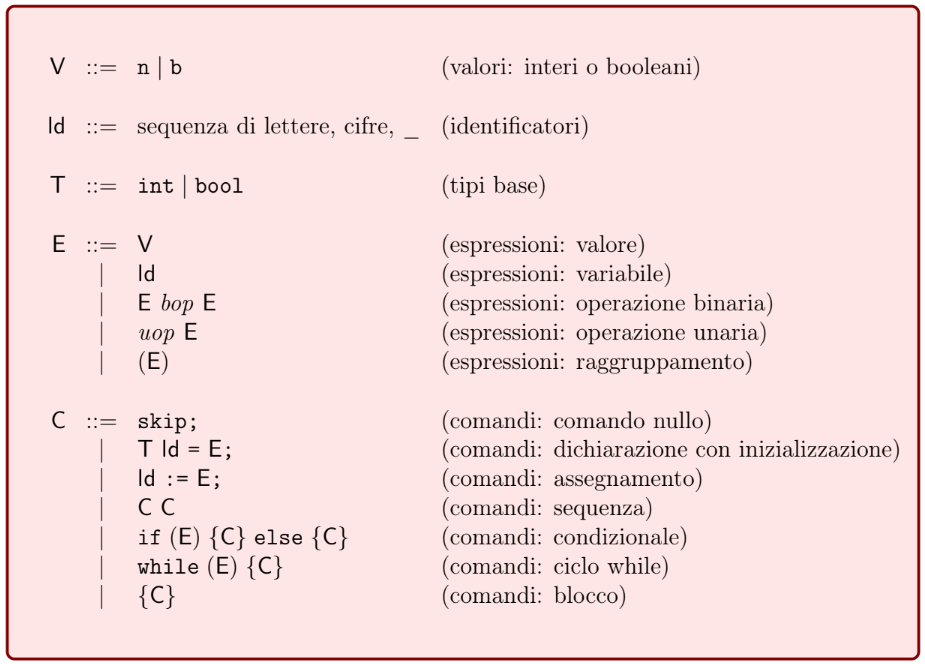
\includegraphics[width=0.9\textwidth]{images/MiniMao_Grammar.png} % replace with your file name
    \caption{Grammatica di MiniMao}
    \label{fig:GrammaticaMiniMao}
\end{figure}
\begin{figure}[h]
    \centering
    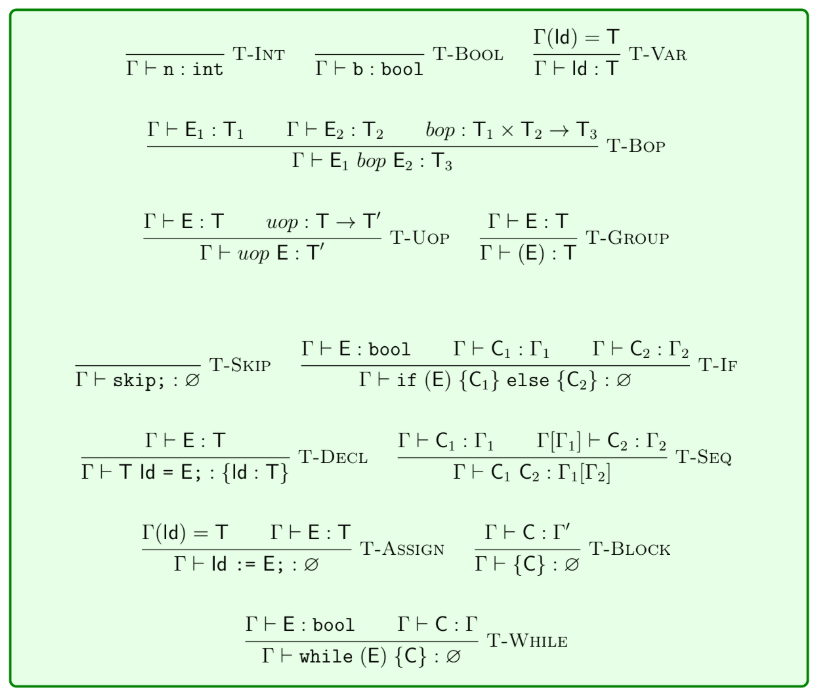
\includegraphics[width=0.9\textwidth]{images/MiniMao_TypeChecking.png} % replace with your file name
    \caption{Type Checking di MiniMao}
    \label{fig:TypeCheckingMiniMao}
\end{figure}
\begin{figure}[h]
    \centering
    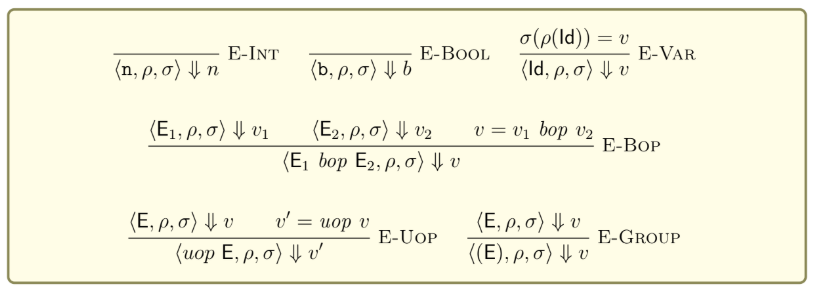
\includegraphics[width=0.9\textwidth]{images/MiniMao_Semantics.png} % replace with your file name
    \caption{Semantica delle espressioni di MiniMao}
    \label{fig:SemanticaMiniMao1}
\end{figure}
\begin{figure}[h]
    \centering
    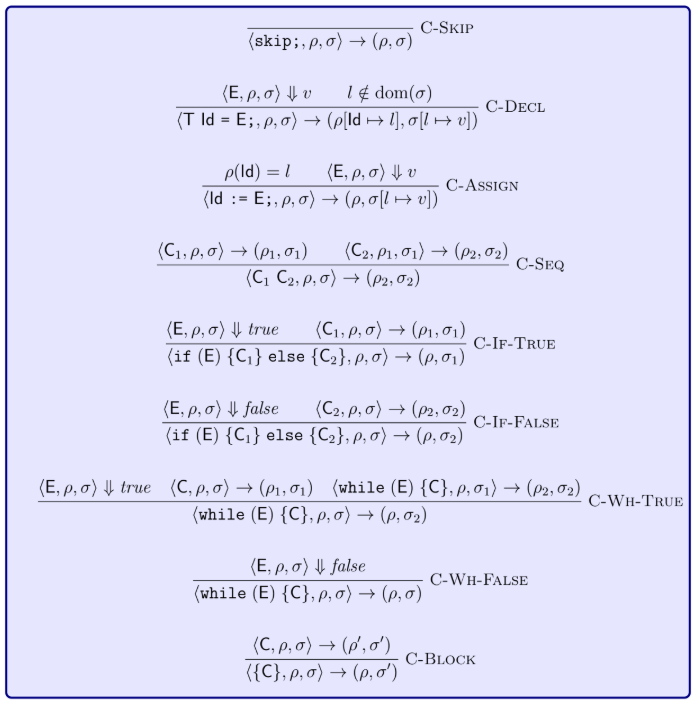
\includegraphics[width=0.9\textwidth]{images/MiniMao_Semantics_Commands.png} % replace with your file name
    \caption{Semantica dei comandi di MiniMao}
    \label{fig:SemanticaMiniMao2}
\end{figure}

\begin{figure}[h]
    \centering
    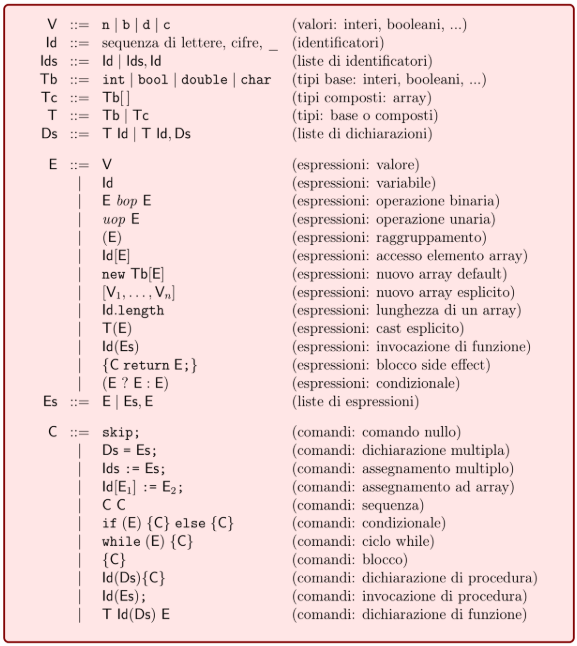
\includegraphics[width=0.9\textwidth]{images/Mao_Grammar.png} % replace with your file name
    \caption{Grammatica di Mao}
    \label{fig:GrammaticaMao}
\end{figure}
\begin{figure}[h]
    \centering
    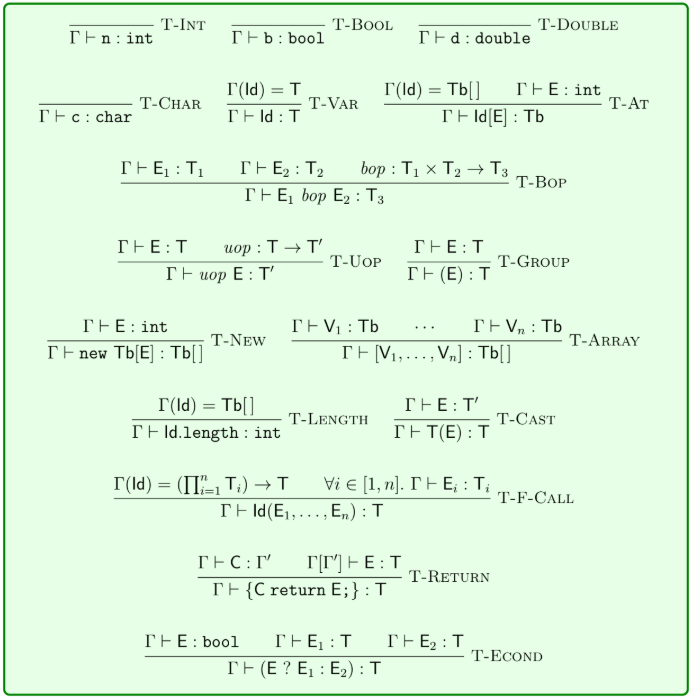
\includegraphics[width=0.9\textwidth]{images/Mao_TypeChecking.png} % replace with your file name
    \caption{Type Checking delle espressioni di Mao}
    \label{fig:TypeCheckingExpressionsMao}
\end{figure}
\begin{figure}[h]
    \centering
    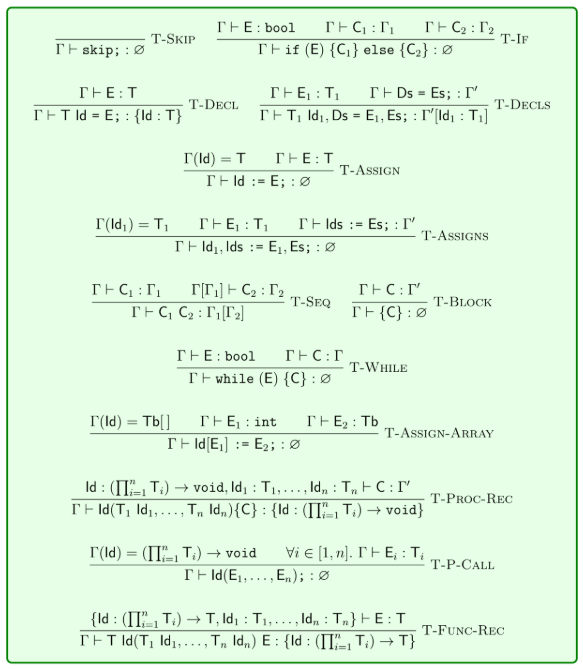
\includegraphics[width=0.9\textwidth]{images/Mao_TypeChecking2.png} % replace with your file name
    \caption{TypeChecking dei comandi di Mao}
    \label{fig:TypeCheckingCommandsMao}
\end{figure}
\begin{figure}[h]
    \centering
    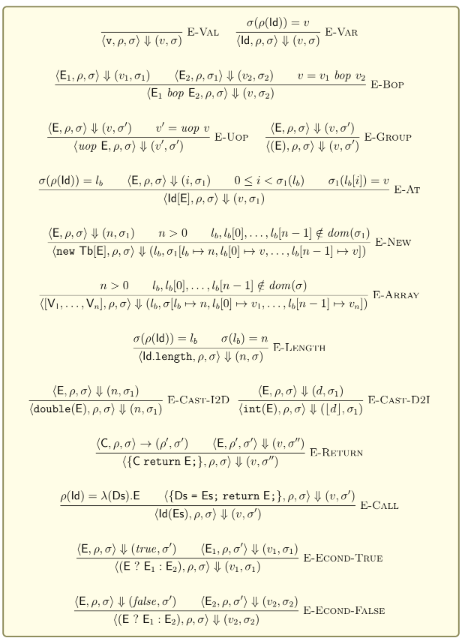
\includegraphics[width=0.9\textwidth]{images/Mao_Semantics1.png} % replace with your file name
    \caption{Semantica delle espressioni di Mao}
    \label{fig:SemanticaEspressioniMao}
\end{figure}
\begin{figure}[h]
    \centering
    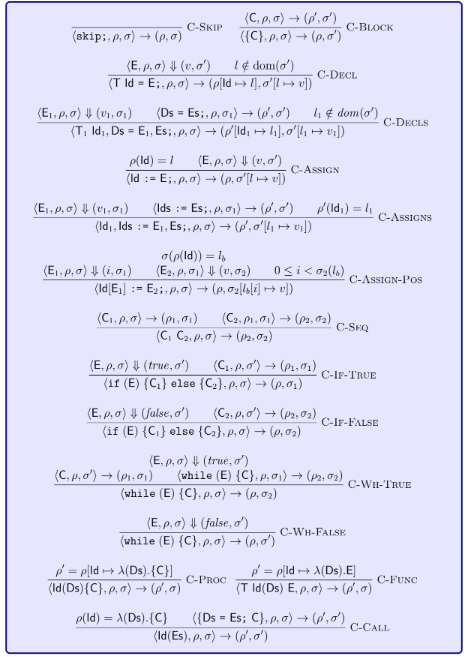
\includegraphics[width=0.9\textwidth]{images/Mao_Semantics2.png} % replace with your file name
    \caption{Semantica dei comandi di Mao}
    \label{fig:SemanticaComandiMao}
\end{figure}


\section{Altro}
La condizione da controllare nei comandi condizionali si chiama \textbf{guardia}.
\end{document}
